\chapter{هندسهٔ مدل}
\label{app:model-geometry}

این پیوست به خواص هندسی و اطلاعاتی بازنمایی‌های حاصل از گشت، مراکز طبقه‌ها و معیارهای ارزیابی کیفیت آن‌ها اختصاص دارد. تعریف بازنمایی‌ها، مراکز و سنجه‌های ناهمانندی در متن اصلی فصل سوم آمده است و خواص عمومی سنجه‌های توزیع‌های احتمال در پیوست~\ref{app:probability-dissimilarity} بررسی شده‌اند. در اینجا روابط تکمیلی معیارهای تراکم درون‌طبقه‌ای، تمایز مراکز و ارتباط این دو با هندسهٔ تصمیم را گردآوری می‌کنیم.

\section{خواص نظری و روابط تکمیلی معیارهای تراکم و جدایی}
\label{cmp:sec:ch3-quality-criteria-theory}
این بخش هویت‌های آنتروپی، کران‌ها، روابط مقایسه‌ای و شرایط برابری معیارهای معرفی‌شده در بخش~\ref{cmp:sec:ch3-quality-criteria} را گردآوری می‌کند. اثبات‌های تفصیلی در بخش‌های بعدی همین پیوست ارائه شده‌اند.

\subsection{هویت‌ها و کران‌های معیارهای تراکم}
هویت عمومی آنتروپی مخلوط، تعبیر هزینهٔ تجمیع و
کران‌های تراکم KL در بخش‌های~\ref{app:ch3-entropy-mixture}
و~\ref{app:ch3-compactness-entropy-relations} اثبات
می‌شوند. در همان بخش، رابطهٔ تراکم مرکزی و زوجی
جنسن--شنون با هزینهٔ تجمیع از طریق میانگین‌های جفتی
استخراج می‌شود. در ادامه، خواص هندسی و متریکی
تکمیلی این معیارها را بررسی می‌کنیم.

\paragraph{تجزیهٔ هیلبرتی تراکم مرکزی و زوجی.}
\phantomsection\label{app:geometry-js-hilbert-dispersion}
برای طبقهٔ غیرتهی $C_c$، با استفاده از نمایش هیلبرتی
متریک جذر جنسن--شنون، $x_i=\Phi(\mathscr Y_i)$ و
میانگین $\overline{\Phi}_c$ تعریف‌شده در
رابطه~\eqref{cmp:eq:ch3-js-hilbert-mean} را در نظر می‌گیریم. برای هر $z\in\mathcal H$، با بسط
مربع هنجار و استفاده از
$\sum_{i\in C_c}(x_i-\overline{\Phi}_c)=0$ داریم:
\[
\frac1{|C_c|}\sum_{i\in C_c}\|x_i-z\|_{\mathcal H}^{2}
=\frac1{|C_c|}\sum_{i\in C_c}\|x_i-\overline{\Phi}_c\|_{\mathcal H}^{2}
+\|\overline{\Phi}_c-z\|_{\mathcal H}^{2}.
\]
به همین ترتیب، با بسط مربع فاصلهٔ زوج‌ها حول
$\overline{\Phi}_c$ و حذف جمله‌های متقاطع داریم:
\[
R_{c,\mathrm{JS}}^{\mathrm{pair}}
=\frac1{|C_c|^2}\sum_{i,j\in C_c}\|x_i-x_j\|_{\mathcal H}^{2}
=\frac2{|C_c|}\sum_{i\in C_c}\|x_i-\overline{\Phi}_c\|_{\mathcal H}^{2}.
\]
با قرار دادن $z=\Phi(\mathcal V_c)$ در هویت نخست
و جایگذاری هویت دوم، نتیجه می‌شود:
\[
R_{c,\mathrm{JS}}=\frac12R_{c,\mathrm{JS}}^{\mathrm{pair}}
+\|\Phi(\mathcal V_c)-\overline{\Phi}_c\|_{\mathcal H}^{2},
\]
که همان رابطه~\eqref{cmp:eq:ch3-js-hilbert-dispersion-decomposition} است.
در رابطهٔ اخیر، جملهٔ دوم مربع فاصلهٔ میانگین حسابی نگاشت توزیع‌ها
از نگاشت میانگین حسابی توزیع‌ها در فضای هیلبرت است.
$\overline{\Phi}_c$ کمینه‌کنندهٔ یکتای میانگین مربع
فاصله در کل فضای هیلبرت است، اما لزوماً در تصویر
سیمپلکس تحت $\Phi$ قرار ندارد.

اگر مرکز به‌جای کل فضای هیلبرت به فضای توزیع‌های
احتمال محدود باشد، با قرار دادن $z=\Phi(Q)$ برای
هر $Q\in\Delta_K$ در همان هویت، داریم:
\[
\frac1{|C_c|}\sum_{i\in C_c}\operatorname{JSD}(\mathscr Y_i,Q)
=\frac12 R_{c,\mathrm{JS}}^{\mathrm{pair}}
+\|\Phi(Q)-\overline{\Phi}_c\|_{\mathcal H}^{2}.
\]
از آنجا که جملهٔ نخست مستقل از $Q$ است، نتیجه می‌شود:
\begin{equation}\label{cmp:eq:ch3-js-optimal-center-projection}
\boxed{\begin{aligned}
&\underset{Q\in\Delta_K}{\arg\min}\;
\frac1{|C_c|}\sum_{i\in C_c}\operatorname{JSD}(\mathscr Y_i,Q)\\
&\qquad=\underset{Q\in\Delta_K}{\arg\min}\;
\|\Phi(Q)-\overline{\Phi}_c\|_{\mathcal H}^{2}.
\end{aligned}}
\end{equation}
بنابراین تعیین مرکز بهینه برای میانگین واگرایی
جنسن--شنون معادل یافتن نزدیک‌ترین نقطه از تصویر
سیمپلکس $\Phi(\Delta_K)$ به میانگین حسابی تصاویر
است. به‌دلیل فشردگی $\Delta_K$ و پیوستگی نگاشت
$\Phi$ (که از رابطهٔ ایزومتری و پیوستگی JSD حاصل
می‌شود)، چنین نقطه‌ای وجود دارد. این مسئله با
کمینه‌سازی میانگین خود فاصلهٔ جذر جنسن--شنون، که
مسئلهٔ میانهٔ هندسی مقید به تصویر سیمپلکس است، و
با کمینه‌سازی بیشترین فاصله، که مسئلهٔ پوشش است،
تفاوت دارد. در نتیجه مفهوم مرکز بهینه به تابع هدف
و فضای مجاز انتخاب مرکز وابسته است؛ این بحث تغییری
در قرارداد مرکز حسابی اصلی مدل ایجاد نمی‌کند.

نامنفی بودن جملهٔ دوم نشان می‌دهد
$R_{c,\mathrm{JS}}^{\mathrm{pair}}\le 2R_{c,\mathrm{JS}}$؛
تساوی دقیقاً هنگامی برقرار است که
$\Phi(\mathcal V_c)=\overline{\Phi}_c$.
از رابطه~\eqref{cmp:eq:ch3-R-JS-KL-midpoint-identity}
و نامنفی بودن $R_{B,c}$ نیز نتیجه می‌شود
$2R_{c,\mathrm{JS}}=R_c-2R_{B,c}\le R_c$.
تساوی در نامساوی دوم دقیقاً هنگامی برقرار است که
$R_{B,c}=0$، یعنی برای همهٔ اعضای طبقه
$\mathscr B_{c,i}=\mathcal V_c$ و در نتیجه
$\mathscr Y_i=\mathcal V_c$.
با توجه به $R_c=R_{c,\mathrm{KL}}$،
زنجیرهٔ رابطه~\eqref{cmp:eq:ch3-js-compactness-chain}
ثابت می‌شود.

\paragraph{واریانس فاصله‌ها و رابطهٔ صورت‌های مبتنی بر متریک.}
در روابط~\eqref{cmp:eq:ch3-js-central-distance-variance}
و~\eqref{cmp:eq:ch3-js-pair-distance-variance}، واریانس
تجربی با وزن‌های یکسان (نه برآورد اصلاح‌شدهٔ نمونه‌ای)
به کار می‌رود. هویت $\operatorname{Var}(D)=
\mathbb E[D^2]-(\mathbb E[D])^2$ با انتخاب $D$ به‌عنوان
فاصلهٔ متریک نمونه تا مرکز یا فاصلهٔ یک زوج مرتب
از اعضای طبقه، به‌ترتیب دو رابطهٔ یادشده را نتیجه
می‌دهد. در صورت زوجی، زوج‌های خودی نیز با وزن
$1/|C_c|^2$ لحاظ می‌شوند. واریانس فاصله تا مرکز
میزان ناهمگنی شعاع‌ها را اندازه می‌گیرد، نه پراکندگی
جهت‌های بازنمایی‌ها در فضای هیلبرت.

از نامساوی مثلثی متریک جذر جنسن--شنون برای هر
$i,j\in C_c$ داریم:
\[
d_{\sqrt{\mathrm{JS}}}(\mathscr Y_i,\mathscr Y_j)
\le d_{\sqrt{\mathrm{JS}}}(\mathscr Y_i,\mathcal V_c)
+d_{\sqrt{\mathrm{JS}}}(\mathscr Y_j,\mathcal V_c).
\]
با میانگین‌گیری روی همهٔ زوج‌های مرتب، هر یک از دو
جملهٔ سمت راست به $R_{c,\sqrt{\mathrm{JS}}}$ تبدیل
می‌شود و رابطه~\eqref{cmp:eq:ch3-js-root-pair-inequality}
به دست می‌آید.

\paragraph{تعبیر شباهتی معیارهای تجمیع‌شده.}
با میانگین‌گیری از
رابطه~\eqref{cmp:eq:ch3-js-compactness-distance-similarity}
روی اعضای یک طبقه یا همهٔ زوج‌های مرتب، به‌ترتیب
روابط~\eqref{cmp:eq:ch3-js-central-similarity}
و~\eqref{cmp:eq:ch3-js-pair-similarity} به دست می‌آیند.
با تعریف میانگین وزن‌دار شباهت درون‌طبقه‌ای
\[
\overline s_{\mathrm{in}}=
\sum_{c=1}^K\frac{\omega_c}{|C_c|}
\sum_{i\in C_c}s(\mathscr Y_i,\mathcal V_c),
\]
داریم:
\begin{equation}\label{cmp:eq:ch3-R-JS-similarity-interpretation}
\begin{aligned}
R_{\mathrm{JS}}&=\log2\,(1-\overline s_{\mathrm{in}}),\\
R_{\sqrt{\mathrm{JS}}}&=\sqrt{\log2}
\sum_{c=1}^K\frac{\omega_c}{|C_c|}
\sum_{i\in C_c}\sqrt{1-s(\mathscr Y_i,\mathcal V_c)}.
\end{aligned}
\end{equation}
بنابراین، میانگین شباهت نرمال‌شده و میانگین JSD
اطلاعات یکسانی ارائه می‌کنند؛ اما میانگین خود فاصلهٔ
متریک به‌طور کلی از میانگین شباهت به‌تنهایی به دست
نمی‌آید.

\paragraph{تعبیر و مقایسه معیارهای تراکم.}
$R_{\mathrm{KL}}$ هزینه اضافی مدل مشترک
برای توزیع‌های یک طبقه را می‌سنجد؛
هرچند KL به‌طور کلی جهت‌دار و بالقوه نامتناهی است،
$R_c$ در این مسئله به‌دلیل انتخاب مرکز حسابی
همواره متناهی و طبق
رابطه~\eqref{cmp:eq:ch3-R-KL-bounds}
کراندار است. تعبیر آن از هویت
آنتروپی مخلوط حاصل می‌شود؛
رابطه~\eqref{cmp:eq:ch3-R-JS-KL-midpoint-identity}
نیز نشان می‌دهد معیار JS تعبیر
آنتروپی مرتبط ولی متفاوتی دارد.
در مقابل، $R_{\mathrm{JS}}$ میانگین
\emph{مربع فاصله متریک} و
$R_{\sqrt{\mathrm{JS}}}$ میانگین
\emph{خود فاصله متریک} نمونه‌ها
از مراکز طبقات است. بنابراین اولی
انحراف‌های دورتر را به‌صورت مربعی
و دومی فاصله‌ها را به‌صورت خطی
در میانگین وارد می‌کند.
با درنظرگرفتن توزیع وزنی نمونه‌ها
که وزن هر عضو طبقه $c$ در آن
$\omega_c/|C_c|$ است،
از ینسن و کرانداری
$d_{\sqrt{\mathrm{JS}}}\le\sqrt{\log2}$
به‌دست می‌آید:
\[
\bigl(R_{\sqrt{\mathrm{JS}}}\bigr)^2
\le R_{\mathrm{JS}}
\le \sqrt{\log2}\,R_{\sqrt{\mathrm{JS}}}.
\]
نامساوی نخست از
$(\mathbb E[d])^2\le\mathbb E[d^2]$
و دومی از $d^2\le\sqrt{\log2}\,d$
نتیجه می‌شود.
این پیوند به معنای
یکسان‌بودن معیارها یا اثرشان
در بهینه‌سازی نیست.
همچنین میانگین حسابی طبقه،
اگرچه برای $R_{\mathrm{KL}}$ بهینه است،
لزوماً کمینه‌کننده
$R_{\mathrm{JS}}$ یا
$R_{\sqrt{\mathrm{JS}}}$ نیست.
پس مقدارهای این سه معیار
هم‌واحد نیستند و مقایسه عددی‌شان
بدون توجه به تعبیر و مقیاس
موجه نخواهد بود.


\paragraph{چرا کمینه‌سازی $R$ به‌تنهایی کافی نیست؟}
معیارهای مرکزی KL و جنسن--شنون فقط نزدیک‌شدن توزیع‌ها \emph{درون هر طبقه} را می‌سنجند و هیچ شرط مستقیمی بر تمایز مراکز طبقات مختلف تحمیل نمی‌کند. برای مثال، فرض کنیم سیاستی موجب شود همه نمونه‌ها، بدون توجه به برچسب آغازین، توزیع همسایگی یکسانی مانند $q$ داشته باشند:
\begin{equation}\label{cmp:eq:ch3-R-collapse}
\mathscr Y_i=q\quad(\forall i)
\quad\Longrightarrow\quad
\mathcal V_1=\cdots=\mathcal V_K=q
\quad\Longrightarrow\quad
R_{\mathrm{KL}}=R_{\mathrm{JS}}=R_{\sqrt{\mathrm{JS}}}=0.
\end{equation}
در این وضعیت، هر سه معیار تراکم به کمترین مقدار ممکن رسیده‌اند، اما بازنمایی‌های حاصل با قرارداد ثابت آموزشی هیچ تمایزی میان طبقه‌ها نشان نمی‌دهند. بنابراین \emph{فشردگی درون‌طبقه‌ای} باید در کنار \emph{جدایی مراکز طبقات} بررسی شود. 

\subsection{خواص نظری و روابط معیارهای جدایی}
\paragraph{مقایسه چهار معیار.}
اگر هدف معیارهای خطی را بیشینه و هدف معیارهای لگاریتمی را کمینه در نظر بگیریم، روابط زیر همواره برقرارند:
\begin{equation}\label{cmp:eq:ch3-four-criteria-comparison}
\boxed{
\begin{gathered}
T(\mathcal V)\le BT(\mathcal V),\qquad
BTNL(\mathcal V)\le TNL(\mathcal V),\\
TNL(\mathcal V)\ge-\log T(\mathcal V),\qquad
BTNL(\mathcal V)\ge-\log BT(\mathcal V).
\end{gathered}}
\end{equation}
دو نامساوی نخست حاصل مجاز بودن جایگشت همانی در مسئله انتساب و دو نامساوی بعدی حاصل تقعر لگاریتم هستند. شرط مثبت بودن وزن طبقات تضمین می‌کند که $T=1$ و $TNL=0$ فقط در ماتریس همانی، و $BT=1$ و $BTNL=0$ فقط در ماتریس‌های جایگشتی رخ دهند. بااین‌حال، یکسان بودن جواب‌های ایده‌آل به معنای یکسان بودن رتبه‌بندی حالت‌های میانی نیست: معیار لگاریتمی در برابر یک احتمال کوچک حساس‌تر است و بهترین جایگشت در $BT$ لزوماً با بهترین جایگشت در $BTNL$ یکسان نیست. اثبات دقیق نامساوی‌ها و شرایط تساوی در بخش~\ref{app:ch3-four-criteria-comparison} از پیوست~\ref{app:model-geometry} آمده است.

\paragraph{تجزیه بر حسب آنتروپی مراکز.}
اگر $H(U)=-\sum_{d=1}^{K}U(d)\log U(d)$ آنتروپی توزیع احتمال $U$ باشد، هویت آنتروپی مخلوط که پیش‌تر برای تعبیر $R$ به کار رفت، اکنون با انتخاب توزیع‌های $\mathcal V_c$ و وزن‌های $\omega_c$ نتیجه می‌دهد:
\begin{equation}\label{cmp:eq:ch3-I-entropy}
\boxed{I(\mathcal V)=H(\overline{\mathcal V})
-\sum_{c=1}^{K}\omega_c H(\mathcal V_c).}
\end{equation}
اثبات این هویت مشترک در بخش~\ref{app:ch3-entropy-mixture} از پیوست~\ref{app:model-geometry} آمده است.
در این رابطه، افزایش آنتروپی میانگین مراکز و کاهش میانگین آنتروپی خود مراکز هر دو می‌توانند مقدار $I$ را افزایش دهند. بااین‌حال، این دو جمله مستقل از یکدیگر نیستند؛ زیرا میانگین مراکز از خود آن‌ها ساخته شده است.

\paragraph{حد پایین و بالای $I$.}
از تعریف اطلاعات متقابل، می‌توان عدم‌قطعیت باقی‌مانده درباره طبقه آغازین پس از مشاهده برچسب همسایگی را به‌صورت زیر بیان کرد:
\begin{equation}\label{cmp:eq:ch3-I-conditional}
\boxed{I(\mathcal V)=H(C_0)-H(C_0\mid C_\xi)
=H(\Omega)-H(C_0\mid C_\xi).}
\end{equation}
برای روشن شدن منشأ این هویت، توجه می‌کنیم که طبق رابطه~\eqref{cmp:eq:ch3-I-joint-distribution}، در هر برچسب مشاهده‌شده $d$ با احتمال مثبت، احتمال شرطی طبقه آغازین برابر
$\mathrm P(C_0=c\mid C_\xi=d)=\omega_c\mathcal V_{cd}/\overline{\mathcal V}(d)$ است. با جایگذاری این احتمال در تعریف آنتروپی شرطی و باز کردن لگاریتم کسر، یک جمله برابر $H(\Omega)$ و جمله دیگر برابر منفی اطلاعات متقابل در رابطه~\eqref{cmp:eq:ch3-I-mutual-info} می‌شود. محاسبه جبری این تساوی در بخش~\ref{app:ch3-I-bounds-proof} از پیوست~\ref{app:model-geometry} نیز آمده است.

از نامنفی بودن اطلاعات متقابل و آنتروپی شرطی در رابطه~\eqref{cmp:eq:ch3-I-conditional}، و نیز از بیشینه بودن آنتروپی توزیع یکنواخت بر روی $K$ طبقه، نتیجه می‌شود:
\begin{equation}\label{cmp:eq:ch3-I-bounds}
\boxed{0\le I(\mathcal V)\le H(\Omega)\le\log K.}
\end{equation}
حد پایین زمانی به‌دست می‌آید که همه مراکز $\mathcal V_c$ برای طبقات دارای وزن مثبت یکسان باشند؛ زیرا در این صورت برچسب مشاهده‌شده هیچ اطلاعاتی درباره طبقه آغازین فراهم نمی‌کند.

اگر همه وزن‌ها مثبت باشند، رسیدن به کران بالای $H(\Omega)$ به این معناست که با دانستن برچسب مشاهده‌شده، طبقه آغازین بدون ابهام مشخص شود. چون تعداد برچسب‌های آغازین و مقصد هر دو $K$ است، این وضعیت دقیقاً برای ماتریس‌های جایگشتی رخ می‌دهد. بنابراین در فضای تمام ماتریس‌های احتمالی سطری، $I$ و $BT$ نقاط بهینه جهانی یکسانی دارند؛ هرچند شکل تابع هدف و رفتار آن‌ها در وضعیت‌های غیرایده‌آل متفاوت است. اثبات دقیق کران‌ها و شرایط تساوی در بخش~\ref{app:ch3-I-bounds-proof} از پیوست~\ref{app:model-geometry} آمده است. البته ممکن است همه این ماتریس‌های بهینه با سیاست انتخاب ویژگیِ قابل یادگیری روی گراف موجود دست‌یافتنی نباشند.

\paragraph{تمایز از معیار پراکندگی $R$.}
قضیه تجزیه KL در بخش~\ref{cmp:subsec:ch3-mean-center-justification} نشان می‌دهد که میانگین وزن‌دار واگرایی توزیع نمونه‌ها از مرکز مشترک $\overline{\mathcal V}$ به دو جزء تجزیه می‌شود:
\begin{equation}\label{cmp:eq:ch3-R-I-decomposition}
\boxed{
\sum_{c=1}^{K}\frac{\omega_c}{|C_c|}
\sum_{i\in C_c}
D_{\mathrm{KL}}\bigl(\mathscr Y_i\|\overline{\mathcal V}\bigr)
=R+I(\mathcal V).
}
\end{equation}
این رابطه تمایز میان دو مفهوم را روشن می‌کند: $R$ میزان پراکندگی توزیع‌های نمونه‌ها حول \emph{مرکز طبقه خودشان} و $I$ میزان جدایی \emph{مراکز طبقات} از میانگین مشترک را اندازه می‌گیرد. کمینه شدن $R$ به‌تنهایی مانع یکسان شدن همه مراکز نمی‌شود؛ در مقابل، مثبت بودن $I$ مستلزم وجود تفاوت میان دست‌کم دو مرکز دارای وزن مثبت است.

\paragraph{ارتباط معیار اطلاعات متقابل با $T$ و $BT$.}
معیار اطلاعات متقابل $I$، تفاوت میان توزیع مشترک طبقه آغازین و برچسب مشاهده‌شده، یعنی $\mathrm P(C_0,C_\xi)$، و توزیع حاصل از فرض استقلال آن‌ها را اندازه می‌گیرد. برای مقایسه این معیار با $T$، لازم نیست تمام زوج‌های ممکن برچسب‌ها را جداگانه بررسی کنیم. کافی است تنها رویداد \emph{برابر بودن دو برچسب} را در نظر بگیریم و سایر حالت‌ها را در یک گروه قرار دهیم. نامساوی پردازش داده‌ها می‌گوید که چنین خلاصه‌سازی‌ای نمی‌تواند واگرایی KL دو توزیع را افزایش دهد؛ بنابراین واگرایی حاصل ازاین‌رویداد ساده، کران پایینی برای $I$ خواهد بود.

متغیر دودویی $B_{\mathrm{eq}}$ را برابر یک می‌گیریم اگر $C_0=C_\xi$ باشد و در غیر این صورت برابر صفر. طبق تعریف~\eqref{cmp:eq:ch3-T-on-V}، احتمال $B_{\mathrm{eq}}=1$ در توزیع مشترک واقعی برابر $T(\mathcal V)$ است. در توزیع فرض استقلال، همین احتمال برابر $q=\sum_{c=1}^{K}\omega_c\overline{\mathcal V}(c)$ خواهد بود. با تبدیل هر دو توزیع به توزیع‌های برنولی متناظر، نتیجه می‌شود:
\begin{equation}\label{cmp:eq:ch3-I-vs-T}
\boxed{
I(\mathcal V)\ge
D_{\mathrm{KL}}\!\left(
\operatorname{Bern}\bigl(T(\mathcal V)\bigr)
\middle\|
\operatorname{Bern}(q)
\right),\qquad
q=\sum_{c=1}^{K}\omega_c\overline{\mathcal V}(c).
}
\end{equation}
در اینجا $\operatorname{Bern}(p)$ توزیع برنولی با احتمال موفقیت $p$ است و $q$، احتمال هم‌برچسب بودن \emph{در فرض استقلال} را نشان می‌دهد؛ نه احتمال واقعی آن را. به‌ویژه، اگر وزن طبقات یکنواخت باشد، از مجموع یک بودن مؤلفه‌های $\overline{\mathcal V}$ داریم $q=1/K$.

معیار $T$ تنها برابر بودن برچسب‌ها را بررسی می‌کند؛ اما در معیار جایگشتی $BT$، برچسب مشاهده‌شده لازم نیست با برچسب طبقه آغازین یکسان باشد. برای هر جایگشت $\sigma$، به‌جای رویداد قبلی، رویداد $B_\sigma=1$ را معادل $C_\xi=\sigma(C_0)$ تعریف می‌کنیم. احتمال این رویداد در توزیع واقعی و در فرض استقلال به‌ترتیب برابر است با:
\begin{equation}\label{cmp:eq:ch3-I-BT-event-probs}
t_\sigma=\sum_{c=1}^{K}\omega_c\mathcal V_{c,\sigma(c)},
\qquad
q_\sigma=\sum_{c=1}^{K}\omega_c\overline{\mathcal V}\bigl(\sigma(c)\bigr).
\end{equation}
همان استدلال پردازش داده‌ها برای هر جایگشت برقرار است و $I(\mathcal V)\ge D_{\mathrm{KL}}(\operatorname{Bern}(t_\sigma)\|\operatorname{Bern}(q_\sigma))$ را نتیجه می‌دهد. در حالت وزن‌های یکنواخت $\omega_c=1/K$، چون $\sigma$ یک جایگشت است، جمع احتمال‌های مقصد در $q_\sigma$ برابر یک می‌شود و \emph{برای هر جایگشت} داریم $q_\sigma=1/K$. اگر $\sigma^\star$ جایگشتی باشد که امتیاز $BT$ را بیشینه می‌کند، آنگاه $t_{\sigma^\star}=BT(\mathcal V)$ و در نتیجه:
\begin{equation}\label{cmp:eq:ch3-I-vs-BT}
\boxed{
I(\mathcal V)\ge
D_{\mathrm{KL}}\!\left(
\operatorname{Bern}\bigl(BT(\mathcal V)\bigr)
\middle\|
\operatorname{Bern}(1/K)
\right),\qquad \omega_c=\frac{1}{K}.
}
\end{equation}
این کران ارتباط مشخصی میان دو معیار فراهم می‌کند. در بخش~\ref{cmp:subsubsec:ch3-BT} ثابت کردیم $1/K\le BT(\mathcal V)\le1$. از سوی دیگر، تابع $D_{\mathrm{KL}}(\operatorname{Bern}(x)\|\operatorname{Bern}(1/K))$ روی بازه $[1/K,1]$ اکیداً صعودی است. بنابراین، \textbf{با افزایش $BT$، کران پایین تضمین‌شده برای $I$ نیز افزایش می‌یابد}؛ هرچند از این نتیجه نمی‌توان نتیجه گرفت که مقدار واقعی $I$ در هر مرحله بهینه‌سازی الزاماً افزایش پیدا می‌کند.

در نقطه ایده‌آل $BT(\mathcal V)=1$، سمت راست رابطه~\eqref{cmp:eq:ch3-I-vs-BT} به $\log K$ می‌رسد. چون برای وزن‌های یکنواخت $I(\mathcal V)\le\log K$ است، در این حالت الزاماً $I(\mathcal V)=\log K$ خواهد بود. بدین‌ترتیب، هر دو معیار بر روی مجموعه ماتریس‌های احتمالی سطری، در ماتریس‌های جایگشتی به پاسخ ایده‌آل یکسانی می‌رسند؛ ولی شکل تابع هدف و مسیر بهینه‌سازی آن‌ها می‌تواند متفاوت باشد. اثبات تفصیلی کران‌ها و صعودی بودن آن‌ها در بخش~\ref{app:ch3-I-bounds-proof} از پیوست~\ref{app:model-geometry} آمده است. برای وزن‌های غیریکنواخت نیز کران برنولی با پارامتر $q_\sigma$ برقرار می‌ماند، اما این پارامتر دیگر لزوماً برابر $1/K$ نیست.

\paragraph{ارتباط اطلاعات متقابل با خطای تشخیص.}
یکی از مزایای تعبیر اطلاعاتی معیار $I$ آن است که می‌توان از نتایج شناخته‌شده نظریه اطلاعات، از جمله نامساوی فانو، استفاده کرد. اگر هدف، تشخیص طبقه آغازین $C_0$ تنها با مشاهده برچسب همسایگی $C_\xi$ باشد و $P_e=\mathrm P(\widehat C_0\ne C_0)$ احتمال خطای یک تصمیم‌گیرنده مبتنی بر $C_\xi$ باشد، از هویت~\eqref{cmp:eq:ch3-I-conditional} و نامساوی فانو داریم \cite{CoverThomas2006}:
\begin{equation}\label{cmp:eq:ch3-I-Fano}
\boxed{H(\Omega)-I(\mathcal V)
=H(C_0\mid C_\xi)
\le h_2(P_e)+P_e\log(K-1),}
\end{equation}
که در آن $K\ge2$ و $h_2(p)=-p\log p-(1-p)\log(1-p)$ آنتروپی دودویی است. این نامساوی محدودیتی اطلاعاتی بر خطای تشخیص قرار می‌دهد؛ به‌ویژه، اگر اطلاعات متقابل کوچک باشد، خطای تشخیص نمی‌تواند به‌دلخواه کوچک شود. بااین‌حال، \textbf{فانو کران پایین خطا را فراهم می‌کند، نه کران بالای خطای یک طبقه‌بند معین}. افزون بر این، مشاهده تصادفی $C_\xi$ با در اختیار داشتن کل بردار $\mathscr Y_i$ یکسان نیست. ازاین‌رو این نامساوی را نباید بدون فرض‌های اضافی با کران بالای درست‌نمایی لگاریتمی منفی برای مدل پیش‌بینی مبتنی بر $\mathscr Y_i$ یکی دانست.

در نتیجه، $I$ علاوه بر بیان تمایز میان مراکز، با میزان اطلاعات
قابل استفاده برای تشخیص طبقه نیز ارتباط نظری دارد؛
اما این رابطه به‌تنهایی کیفیت تصمیم‌گیری از روی
تمام بردار بازنمایی و حاشیه تک‌تک نمونه‌ها را تعیین نمی‌کند.

در مجموع، معیار اطلاعات متقابل $I$ بدون تحمیل هم‌برچسب بودن یا انتخاب یک جایگشت خاص، تمایز توزیع‌های نماینده طبقات را اندازه می‌گیرد و مانند چهار معیار پیشین، صرفاً بر اساس $\mathcal V$ قابل محاسبه است. تعبیر اطلاعات متقابل و ارتباط آن با عدم‌قطعیت طبقه آغازین، انگیزه نظری مناسبی برای استفاده از $I$ در ارزیابی و بهبود سیاست انتخاب ویژگی فراهم می‌کند.



\section{بهینگی درست‌نماییِ نماینده مشترک توزیع‌های مخلوط}
\label{app:ch3-mixture-likelihood}

این اثبات، صورت عمومی استدلال درست‌نماییِ مطرح‌شده در رابطه~\eqref{cmp:eq:ch3-mixture-likelihood-optimum} را ارائه می‌کند و به تعریف شعاع درون‌طبقه‌ای وابسته نیست. فرض کنیم مشاهدات در $g$ گروه تولید شده‌اند؛ در گروه $r$، تعداد $n_r$ مشاهده مستقل و هم‌توزیع $Z_{r,1},\ldots,Z_{r,n_r}$ از توزیع احتمال $P_r$ روی یک فضای متناهی داریم. اگر $n=\sum_r n_r$ و در حد $n\to\infty$ نسبت $n_r/n$ به وزن $\eta_r$ میل کند، فرض می‌کنیم $\eta_r\ge0$ و $\sum_r\eta_r=1$؛ گروه‌های با وزن صفر در محاسبات حدی سهمی ندارند.

اگر بدانیم هر مشاهده از کدام توزیع تولید شده، درست‌نمایی مدل آگاه از مبدأ برابر است با
\[
L_n^{\star}=\prod_{r=1}^{g}\prod_{t=1}^{n_r}P_r(Z_{r,t}).
\]
اما اگر لازم باشد همه مشاهدات با یک توزیع مشترک $Q$ توضیح داده شوند، درست‌نمایی آن‌ها برابر است با:
\[
L_n(Q)=\prod_{r=1}^{g}\prod_{t=1}^{n_r}Q(Z_{r,t}).
\]
در حالتی که $Q$ روی تکیه‌گاه همهٔ توزیع‌های گروه‌های مشاهده‌شده، از جمله گروه‌های با وزن حدی صفر، مقدار مثبت داشته باشد، از قانون اعداد بزرگ برای هر گروه نتیجه می‌شود:
\begin{equation}\label{eq:app-ch3-mixture-log-likelihood-ratio}
\begin{aligned}
\lim_{n\to\infty}\frac1n\log\frac{L_n^{\star}}{L_n(Q)}
&=\sum_{r=1}^{g}\eta_r
\sum_{d=1}^{K}P_r(d)\log\frac{P_r(d)}{Q(d)}\\
&=\sum_{r=1}^{g}\eta_rD_{\mathrm{KL}}(P_r\|Q).
\end{aligned}
\end{equation}
این همان تفاوت متوسط لگاریتم درست‌نمایی مدل آگاه از مبدأ و مدل مشترک است. چنانچه $Q$ در مؤلفه‌ای که توزیع مخلوط به آن احتمال مثبت می‌دهد، صفر باشد، مدل مشترک برای مشاهده آن مؤلفه درست‌نمایی صفر خواهد داشت و زیان لگاریتمی آن نامتناهی می‌شود.

اکنون میانگین توزیع‌ها را با $\overline P=\sum_r\eta_rP_r$ تعریف می‌کنیم.

هویت تجزیه میانگین KL که در صورت درون‌طبقه‌ای متن اصلی به کار می‌رود، برای هر توزیع مشترک $Q$ چنین است؛ گروه‌های با وزن صفر از جمع‌ها حذف می‌شوند:
\begin{equation}\label{eq:app-ch3-mixture-KL-general}
\boxed{
\begin{aligned}
\sum_{r=1}^{g}\eta_rD_{\mathrm{KL}}(P_r\|Q)
&=\sum_{r=1}^{g}\eta_rD_{\mathrm{KL}}(P_r\|\overline P)\\
&\quad+D_{\mathrm{KL}}(\overline P\|Q).
\end{aligned}}
\end{equation}
 با افزودن و کاستن $\log\overline P(d)$ در عبارت آخر و جابه‌جا کردن جمع‌ها داریم:
\begin{equation}\label{eq:app-ch3-mixture-KL-decomposition-proof}
\begin{aligned}
\sum_r\eta_rD_{\mathrm{KL}}(P_r\|Q)
&=\sum_r\eta_r\sum_dP_r(d)
\log\frac{P_r(d)}{\overline P(d)}
+\sum_r\eta_r\sum_dP_r(d)
\log\frac{\overline P(d)}{Q(d)}\\
&=\sum_r\eta_rD_{\mathrm{KL}}(P_r\|\overline P)
+\sum_d\overline P(d)\log\frac{\overline P(d)}{Q(d)}\\
&=\sum_r\eta_rD_{\mathrm{KL}}(P_r\|\overline P)
+D_{\mathrm{KL}}(\overline P\|Q).
\end{aligned}
\end{equation}
در مؤلفه‌های صفر از قراردادهای متداول KL استفاده می‌کنیم. این محاسبه در حالت متناهی انجام شده است. اگر $Q$ روی تکیه‌گاه $\overline P$ صفر باشد، هر دو طرف هویت نامتناهی‌اند؛ جملهٔ نخست سمت راست همیشه متناهی است. این هویت همان رابطه~\eqref{cmp:eq:ch3-center-excess-average-kl} را برای وزن‌های برابر نتیجه می‌دهد. عبارت نخست مستقل از $Q$ و عبارت دوم نامنفی است؛ بنابراین کمترین زیان درست‌نماییِ حاصل از استفاده از یک توزیع مشترک، دقیقاً در $Q=\overline P$ به‌دست می‌آید. برابری فقط در همین حالت رخ می‌دهد.

همچنین می‌توان مستقیماً متوسط لگاریتم درست‌نمایی مدل مشترک را محاسبه کرد:
\begin{equation}\label{eq:app-ch3-mixture-MLE-proof}
\begin{aligned}
\mathcal L(Q)
&=\sum_r\eta_r\sum_dP_r(d)\log Q(d)\\
&=\sum_d\overline P(d)\log Q(d)\\
&=-H(\overline P)-D_{\mathrm{KL}}(\overline P\|Q).
\end{aligned}
\end{equation}
بنابراین بیشینه‌کننده $\mathcal L(Q)$ همان $\overline P$ است. این گزاره مبنای \emph{درست‌نمایی} انتخاب میانگین است؛ تجزیه KL فقط راه اثبات آن را فراهم می‌کند.

برای طبقه $c$ در روش پیشنهادی، با قرار دادن $P_r=\mathscr Y_i$ برای $i\in C_c$ و وزن‌های $\eta_r=1/|C_c|$، نتیجه می‌شود که بهترین توزیع مشترک برای مدل‌کردن مشاهدات برچسب همسایگی نمونه‌های این طبقه، همان $\mathcal V_c$ است. این نتیجه نه به تعریف $R_c$ وابسته است و نه لزوماً به معنای کمینه‌کننده بودن همین نماینده برای هر فاصله یا متریک دیگری مانند جذر واگرایی جنسن--شنون است.

\paragraph{مقدار بهینه منفی لگاریتم درست‌نمایی و تفسیر هزینه تجمیع.}
برای توزیع مشترک $Q$، منفی لگاریتم درست‌نمایی مورد انتظار برابر $-\mathcal L(Q)$ است؛ بنابراین با استفاده از رابطه~\eqref{eq:app-ch3-mixture-MLE-proof}، کمترین مقدار آن در $Q=\overline P$ برابر $H(\overline P)$ خواهد بود. اگر به‌جای یک مدل مشترک، مدل جداگانه $Q_r$ برای مشاهده‌های گروه $r$ در اختیار داشته باشیم، هزینه هر گروه از رابطه
\[
-\sum_d P_r(d)\log Q_r(d)
=H(P_r)+D_{\mathrm{KL}}(P_r\|Q_r)
\]
به‌دست می‌آید. این هزینه برای $Q_r=P_r$ کمینه می‌شود؛ ازاین‌رو کمترین هزینه میانگین مدل‌های اختصاصی $\sum_r\eta_rH(P_r)$ است. در نتیجه اختلاف دو مقدار بهینه برابر است با:
\begin{equation}\label{eq:app-ch3-NLL-compression-gap}
\begin{aligned}
\operatorname{NLL}_{\min}^{\mathrm{shared}}
-\operatorname{NLL}_{\min}^{\mathrm{individual}}
&=H(\overline P)-\sum_r\eta_rH(P_r)\\
&=\sum_r\eta_rD_{\mathrm{KL}}(P_r\|\overline P)
\ge0.
\end{aligned}
\end{equation}
تساوی دوم، نمونه‌ای از \emph{هویت عمومی آنتروپی مخلوط}
است که در بخش~\ref{app:ch3-entropy-mixture} به‌صورت
یک گزاره مستقل اثبات می‌کنیم؛ در اینجا تنها
کاربرد آن برای تفسیر تفاوتِ بهینه دو مدل
درست‌نمایی موردنظر است. اگر همه وزن‌های مورد بحث
مثبت باشند، اختلاف هزینه دقیقاً زمانی صفر است
که تمام $P_r$ها برابر باشند. این هزینه تنها
درباره پیش‌بینی \emph{مشاهداتِ مولد از توزیع‌های $P_r$}
است؛ بنابراین نباید با منفی لگاریتم درست‌نمایی
برچسب واقعی نمونه آغازین در مسئله طبقه‌بندی
یکی گرفته شود.

\paragraph{صورت دقیق تجزیه برای یک طبقه.}
برای طبقه $c$، در رابطه~\eqref{eq:app-ch3-mixture-KL-general} به‌ترتیب $P_r=\mathscr Y_i$، $\eta_r=1/|C_c|$، $\overline P=\mathcal V_c$ و $Q=U$ قرار می‌دهیم. در این صورت برای هر $U$ با واگرایی‌های متناهی:
\begin{equation}\label{eq:ch3-KL-proof}
\begin{aligned}
\frac1{|C_c|}\sum_{i\in C_c}
D_{\mathrm{KL}}(\mathscr Y_i\|U)
&=\frac1{|C_c|}\sum_{i\in C_c}
D_{\mathrm{KL}}(\mathscr Y_i\|\mathcal V_c)\\
&\quad+\sum_d
\left(\frac1{|C_c|}\sum_{i\in C_c}\mathscr Y_i(d)\right)
\log\frac{\mathcal V_c(d)}{U(d)}\\
&=R_c+D_{\mathrm{KL}}(\mathcal V_c\|U).
\end{aligned}
\end{equation}
این همان قضیه~\ref{cmp:thm:ch3-KL-decomposition} است. چون برای هر مؤلفه $d$، برابری $\mathcal V_c(d)=0$ همراه با نامنفی‌بودن $\mathscr Y_i(d)$ها مستلزم $\mathscr Y_i(d)=0$ برای همه اعضای طبقه است، جمله‌های دارای مؤلفه صفر را می‌توان با قرارداد معمول KL محاسبه کرد. اگر در مؤلفه‌ای $\mathcal V_c(d)>0$ اما $U(d)=0$ باشد، هر دو طرفِ عبارت مربوط به مدل $U$ نامتناهی‌اند و تفسیر مستقیم لگاریتم درست‌نمایی برقرار نیست؛ به همین دلیل قضیه با شرط متناهی‌بودن واگرایی‌ها بیان شده است. نامنفی‌بودن $D_{\mathrm{KL}}(\mathcal V_c\|U)$ ثابت می‌کند که نماینده بهینه دقیقاً $\mathcal V_c$ است. همچنین در این صورت، هویت~\eqref{cmp:eq:ch3-R-entropy} تفسیرِ هزینه تجمیع را در قالب آنتروپی و میانگین KL ارائه می‌کند.

\paragraph{هزینه مدل‌کردن یک طبقه با توزیع مشترک.}
با استفاده از مرکز حسابی تعریف‌شده در رابطه~\eqref{cmp:eq:ch3-class-center} و توجیه درست‌نمایی آن در بخش~\ref{cmp:subsec:ch3-mean-center-justification}، برای طبقهٔ $c$، با وزن‌های یکسان $1/|C_c|$، \emph{کمترین میانگین منفی لگاریتم درست‌نمایی مورد انتظار} برای مدل مشترک به‌دست می‌آید:
\begin{equation}\label{cmp:eq:ch3-class-shared-NLL}
\boxed{\operatorname{NLL}^{\mathrm{shared}}_{c,\min}
=H(\mathcal V_c).}
\end{equation}
برای مقایسه، اگر توزیع مولد اختصاصی هر مشاهده معلوم باشد و مشاهدات متناظر با $\mathscr Y_i$ را با خود همان توزیع مدل کنیم، کمترین هزینه مورد انتظار برابر است با:
\begin{equation}\label{cmp:eq:ch3-class-individual-NLL}
\boxed{\operatorname{NLL}^{\mathrm{individual}}_{c,\min}
=\frac{1}{|C_c|}\sum_{i\in C_c}H(\mathscr Y_i).}
\end{equation}
اختلاف این دو مقدار، هزینه اضافی \emph{تجمیع} توزیع‌های نمونه‌های طبقه در یک نماینده مشترک را می‌سنجد. این اختلاف را با $R_c$ نشان می‌دهیم:
\begin{equation}
\boxed{
\begin{aligned}
R_c
&=\operatorname{NLL}^{\mathrm{shared}}_{c,\min}
-\operatorname{NLL}^{\mathrm{individual}}_{c,\min}\\
&=H(\mathcal V_c)
-\frac1{|C_c|}\sum_{i\in C_c}H(\mathscr Y_i)\\
&=\frac1{|C_c|}\sum_{i\in C_c}
D_{\mathrm{KL}}(\mathscr Y_i\|\mathcal V_c).
\end{aligned}}
\end{equation}
برابری آخر از تعریف آنتروپی و میانگین‌بودن $\mathcal V_c$ حاصل می‌شود. بنابراین $R_c\ge0$؛ اگر توزیع همسایگی همه نمونه‌های طبقه یکسان باشد، این هزینه صفر است. برای مثال، دو توزیع $(1,0)$ و $(0,1)$ و نیز دو توزیع یکسان $(1/2,1/2)$ هر دو مرکز $(1/2,1/2)$ دارند؛ اما هزینه تجمیع در حالت اول $\log2$ و در حالت دوم صفر است. پس آنتروپی مرکز به‌تنهایی پراکندگی توزیع‌های اعضای طبقه را مشخص نمی‌کند.

\paragraph{اثر انتخاب نماینده‌ای غیر از میانگین.}
هویت زیر نشان می‌دهد در صورت انتخاب یک توزیع مشترک دیگر مانند $U$، علاوه بر هزینه اجتناب‌ناپذیر تجمیع، هزینه‌ای اضافی نیز پرداخت می‌شود:
\begin{theorem}[تجزیه هزینه مدل‌سازی مشترک]\label{cmp:thm:ch3-KL-decomposition}
برای هر طبقه $c$ و هر توزیع احتمال $U$ که واگرایی‌های مربوط به آن متناهی باشند، داریم:
\begin{equation}\label{cmp:eq:ch3-KL-decomposition}
\boxed{
\frac{1}{|C_c|}\sum_{i\in C_c}
D_{\mathrm{KL}}(\mathscr Y_i\|U)
=R_c+D_{\mathrm{KL}}(\mathcal V_c\|U).}
\end{equation}
\end{theorem}
در نتیجه، جمله $R_c$ هزینه ناشی از خلاصه‌کردن توزیع‌های متفاوت با \emph{یک} نماینده است و جمله $D_{\mathrm{KL}}(\mathcal V_c\|U)$ زیان اضافیِ برگزیدن نماینده‌ای غیر از میانگین بهینه را نشان می‌دهد. به‌ویژه:
\begin{equation}\label{cmp:eq:ch3-KL-opt-center}
\boxed{\mathcal V_c=
\underset{U}{\arg\min}\;
\frac{1}{|C_c|}\sum_{i\in C_c}
D_{\mathrm{KL}}(\mathscr Y_i\|U).}
\end{equation}
تجزیهٔ عمومی و اثبات صورت درون‌طبقه‌ای این رابطه در همین بخش ارائه شدند.

این تفسیر روشن می‌کند چرا $R_c$ را در ارزیابی بازنمایی اندازه می‌گیریم: این معیار هزینه فشرده‌سازی الگوهای همسایگی هر طبقه در یک توزیع مشترک است. البته این هزینه، \emph{منفی لگاریتم درست‌نماییِ برچسب واقعی نمونه} یا خطای تصمیم طبقه‌بند نیست. ممکن است $R_c$ برای همه طبقه‌ها صفر باشد ولی مراکز آن‌ها نیز با یکدیگر برابر باشند و امکان تفکیک وجود نداشته باشد. بنابراین، بهینگی نمایندگی درون هر طبقه را باید از کیفیت \emph{تمایز میان طبقه‌ها} جدا کرد؛ معیارهای این دو جنبه در ادامه بررسی می‌شوند.

\paragraph{قرارداد تکیه‌گاه KL در برابر هموارسازی عددی.}
\phantomsection\label{cmp:par:ch3-KL-legacy-clip}
در تعریف دقیق از قرارداد $0\log(0/q)=0$ برای $q\ge0$
استفاده می‌شود و هرگاه $p_u>0$ ولی $q_u=0$ باشد،
$D_{\mathrm{KL}}(P\|Q)=+\infty$ است.
برای $R_{\mathrm{KL}}$ که مرکز همان میانگین حسابی
نمونه‌های هر طبقه است، چنین ناسازگاریِ تکیه‌گاه
در جهت $\mathscr Y_i\|\mathcal V_c$ رخ نمی‌دهد
و مقدار معیار متناهی است؛ اما در فاصله نمونه به
\emph{مرکز طبقه رقیب} یا هدف خارجی این تضمین وجود ندارد.
جایگزینی صفرها با کران پایین مثبت در محاسبهٔ
\lr{clip} یک قرارداد عددیِ متفاوت می‌سازد:
$R_{\mathrm{KL}}^{\mathrm{legacy,clip}}$
را نباید بدون باز‌محاسبه با تعریف دقیق
$R_{\mathrm{KL}}$ یکی گرفت. این تفاوت در
تفسیر خروجی‌های ذخیره‌شدهٔ فصل~\ref{chap:results}
اهمیت دارد، نه در درستی هویت‌های دقیقِ KL.

\paragraph{از مشاهدات گشت تا هزینه درست‌نمایی.}
در زیربخش~\ref{cmp:subsec:ch3-mean-center-justification}
دیدیم که مرکز حسابی توزیع‌های
برچسب همسایگی یک طبقه، بهترین
توزیع مشترک برای توضیح مشاهدات
آن طبقه در معنای درست‌نمایی
مورد انتظار است. اثبات این
نتیجه در پیوست~
\ref{app:ch3-mixture-likelihood}
بر مقایسه درست‌نمایی مشاهداتی
استوار بود که از توزیع‌های
متفاوت به دست می‌آیند.
اکنون همان استدلال را برای
\emph{یک نمونه مبدأ} بازخوانی می‌کنیم تا معنای
هزینهٔ KL تک‌نمونه‌ای در پوشش چندکی روشن شود.

فرض کنیم $i\in C_c$ یک نمونه
آموزشی از طبقه $c$ باشد و
$\mathscr Y_i\in\Delta_K$
توزیع برچسب مقصد مشاهده‌شده
در گشت تصادفیِ آغازشده از آن
را، تحت سیاست و قرارداد
توقف ثابت، نشان دهد.
مرکز همان طبقه مطابق
رابطه~\eqref{cmp:eq:ch3-class-center}
برابر است با
$\mathcal V_c=|C_c|^{-1}
\sum_{j\in C_c}\mathscr Y_j$.
برای توضیح برچسب‌های حاصل
از گشت این نمونه، می‌توان
از دو مدل احتمالاتی استفاده کرد:
\emph{توزیع اختصاصی} خود نمونه
یعنی $\mathscr Y_i$، یا
\emph{توزیع مشترک} طبقه
یعنی $\mathcal V_c$.

اگر $Z_{i,1},\ldots,Z_{i,T}$
برچسب‌های حاصل از $T$
\emph{تکرار مستقلِ آزمایش کامل گشت}
از مبدأ $i$ باشند، در قرارداد
مذکور هر $Z_{i,t}$ از
$\mathscr Y_i$ توزیع دارد.
درست‌نمایی این مشاهدات
با مدل اختصاصی و مدل مشترک
به‌ترتیب حاصل‌ضرب احتمال‌های
$\mathscr Y_i(Z_{i,t})$
و $\mathcal V_c(Z_{i,t})$
است. با همان استدلال قانون
اعداد بزرگ در رابطه~
\eqref{eq:app-ch3-mixture-log-likelihood-ratio}
از پیوست، داریم:
\begin{equation}\label{cmp:eq:ch3-outlier-kl-likelihood-decomposition}
\boxed{
\begin{aligned}
&\lim_{T\to\infty}\frac1T
\log\frac{
\prod_{t=1}^{T}\mathscr Y_i(Z_{i,t})
}{
\prod_{t=1}^{T}\mathcal V_c(Z_{i,t})
}\\
&\qquad
=\sum_{u=1}^{K}\mathscr Y_i(u)
\log\frac{\mathscr Y_i(u)}{\mathcal V_c(u)}
=D_{\mathrm{KL}}(\mathscr Y_i\|\mathcal V_c).
\end{aligned}}
\end{equation}
این حد برای تکرارهای مستقل
\emph{گشت کامل} است و به
استقلال گام‌های متوالی
\emph{درون یک گشت} نیازی ندارد.
ازآنجاکه مرکز از میانگین
همین بازنمایی‌ها تشکیل شده،
روی تکیه‌گاه $\mathscr Y_i$
مقدار مثبت دارد و واگرایی
فوق متناهی است.

بنابراین KL در اینجا فقط
یک سنجه اختلاف انتزاعی نیست:
\emph{افت متوسط لگاریتم درست‌نمایی
به‌ازای هر مشاهده برچسب مقصد}
هنگام جایگزین‌کردن توزیع
اختصاصی نمونه با مرکز مشترک
طبقه است. این نتیجه معادل
هویت آنتروپی متقاطع
$-\sum_u\mathscr Y_i(u)
\log\mathcal V_c(u)
=H(\mathscr Y_i)+
D_{\mathrm{KL}}(\mathscr Y_i\|\mathcal V_c)$
نیز هست. منظور، مدل‌کردن
\emph{برچسب‌های مشاهده‌شده در گشت}
است، نه درست‌نمایی برچسب
واقعی نمونه مبدأ یا مقادیر
ویژگی‌های خام.


\section{هویت آنتروپی مخلوط و تعبیر معیارهای R و I}
\label{app:ch3-entropy-mixture}
هویت زیر مبنای مشترک تفسیر آنتروپی
$R_{\mathrm{KL}}$ و $I$ و نیز اختلاف هزینه
درست‌نماییِ مدل مشترک و مدل اختصاصی در
رابطه~\eqref{eq:app-ch3-NLL-compression-gap} است.
برای جلوگیری از تلقی این کاربردها به‌عنوان
چند فرض مستقل، ابتدا هویت را در حالت عمومی
اثبات و سپس دو جایگذاری مربوط به معیارها را
مشخص می‌کنیم.

\begin{proposition}\label{prop:app-ch3-entropy-mixture}
فرض کنیم $P_1,\ldots,P_m$ توزیع‌های احتمال روی
یک فضای متناهی مشترک و $a_1,\ldots,a_m$ وزن‌های
نامنفی با مجموع یک باشند. اگر
$\overline P=\sum_{r=1}^{m}a_rP_r$ و
$H(P)=-\sum_dP(d)\log P(d)$، آنگاه:
\begin{equation}\label{eq:app-ch3-mixture-entropy}
\boxed{
\sum_{r=1}^{m}a_rD_{\mathrm{KL}}(P_r\|\overline P)
=H(\overline P)-\sum_{r=1}^{m}a_rH(P_r).
}
\end{equation}
در جمع وزن‌دار واگرایی‌ها، جمله‌های دارای وزن صفر
حذف می‌شوند. هر دو طرف هویت متناهی و نامنفی‌اند.
\end{proposition}
\begin{proof}
ابتدا تکیه‌گاه مخلوط را در نظر می‌گیریم. برای هر
$r$ با $a_r>0$ و هر مؤلفهٔ $d$ داریم
$\overline P(d)\ge a_rP_r(d)$. بنابراین،
$P_r(d)>0$ مستلزم $\overline P(d)>0$ است و
\[
\operatorname{supp}(\overline P)
=\bigcup_{r:\,a_r>0}\operatorname{supp}(P_r).
\]
پس واگرایی هر توزیع دارای وزن مثبت از مخلوط
متناهی است. خارج از تکیه‌گاه مخلوط، تمام
توزیع‌های دارای وزن مثبت نیز صفرند و سهم آن
مؤلفه‌ها با قرارداد $0\log0=0$ صفر است.

اکنون در جمع‌های زیر، اندیس $r$ را به وزن‌های
مثبت و اندیس $d$ را به تکیه‌گاه مخلوط محدود
می‌کنیم. با بسط تعریف KL و جدا کردن لگاریتم
صورت و مخرج داریم:
\begin{equation}\label{eq:app-ch3-mixture-entropy-proof}
\begin{aligned}
\sum_r a_rD_{\mathrm{KL}}(P_r\|\overline P)
&=\sum_r a_r\sum_d P_r(d)
\log\frac{P_r(d)}{\overline P(d)}\\
&=\sum_r a_r\sum_dP_r(d)\log P_r(d)\\
&\quad-\sum_r a_r\sum_dP_r(d)\log\overline P(d)\\
&=-\sum_r a_r H(P_r)\\
&\quad-\sum_d\left(\sum_r a_rP_r(d)\right)
\log\overline P(d)\\
&=-\sum_r a_rH(P_r)
-\sum_d\overline P(d)\log\overline P(d)\\
&=H(\overline P)-\sum_r a_rH(P_r).
\end{aligned}
\end{equation}
در گام ماقبل آخر، از تعریف مخلوط استفاده شده
است. افزودن مؤلفه‌های خارج از تکیه‌گاه و
توزیع‌های دارای وزن صفر، در جمع‌های آنتروپی
تغییری ایجاد نمی‌کند. نامنفی بودن طرف چپ
نیز مستقیماً از نامنفی بودن KL نتیجه می‌شود.
به‌علاوه، این مقدار دقیقاً زمانی صفر است که
تمام توزیع‌های دارای وزن مثبت با مخلوط
$\overline P$ یکسان باشند.
\end{proof}

برای معیار شعاع درون‌طبقه‌ای $R_c$، با انتخاب $P_r=\mathscr Y_i$ برای $i\in C_c$ و وزن $1/|C_c|$، مستقیماً رابطه~\eqref{cmp:eq:ch3-R-entropy} به‌دست می‌آید. در گام بعد، با میانگین‌گیری روی طبقه‌ها طبق وزن‌های $\Omega$، تعبیر آنتروپی میانگین $R$ در رابطه~\eqref{cmp:eq:ch3-R-average-entropy} حاصل می‌شود. همچنین با انتخاب $P_r=\mathcal V_c$ و $a_r=\omega_c$، همین گزاره رابطه~\eqref{cmp:eq:ch3-I-entropy} را نتیجه می‌دهد. به این ترتیب، تعبیر آنتروپی $R$ و $I$ دو کاربرد از یک هویت واحدند. صورت تجمیع‌شدهٔ هزینهٔ درون‌طبقه‌ای عبارت است از:
\begin{equation}\label{cmp:eq:ch3-R-average-entropy}
\boxed{R=\sum_{c=1}^{K}\omega_c H(\mathcal V_c)
-\sum_{c=1}^{K}\frac{\omega_c}{|C_c|}
\sum_{i\in C_c}H(\mathscr Y_i).}
\end{equation}
آنتروپی مرکز به‌تنهایی پراکندگی اعضای طبقه را تعیین نمی‌کند؛ اختلاف آن با میانگین آنتروپی بازنمایی‌ها اهمیت دارد.

\subsection{کران تیز هزینه تجمیع و رابطه آن با تراکم جنسن--شنون}
\label{app:ch3-compactness-entropy-relations}
این قسمت دو نتیجه‌ای را که در
بخش~\ref{cmp:subsec:ch3-within-class-compactness}
بیان شدند، از هویت عمومی
\eqref{eq:app-ch3-mixture-entropy}
استخراج می‌کند: کران تراکم KL
و رابطه دقیق میان تراکم KL و جنسن--شنون.

\paragraph{کران $R_c$ و حالت‌های تساوی.}
چون $\mathcal V_c$ میانگین توزیع‌های
$\mathscr Y_i$ برای $i\in C_c$ است،
با جایگذاری در هویت آنتروپی مخلوط داریم:
\begin{equation}\label{eq:app-ch3-R-entropy-bound-proof}
\begin{aligned}
R_c
&=\frac1{|C_c|}\sum_{i\in C_c}
D_{\mathrm{KL}}(\mathscr Y_i\|\mathcal V_c)
\ge0,\\
R_c
&=H(\mathcal V_c)-\frac1{|C_c|}
\sum_{i\in C_c}H(\mathscr Y_i)\\
&\le H(\mathcal V_c)\le\log K.
\end{aligned}
\end{equation}
صورت خلاصهٔ این کران عبارت است از:
\begin{equation}\label{cmp:eq:ch3-R-KL-bounds}
\boxed{
0\le R_c
=H(\mathcal V_c)
-\frac1{|C_c|}\sum_{i\in C_c}H(\mathscr Y_i)
\le H(\mathcal V_c)\le\log K.
}
\end{equation}
برابری $R_c=0$، به دلیل برابربودن
وزن‌های همه اعضای طبقه و شرط تساوی KL،
دقیقاً معادل برابر بودن تمام
$\mathscr Y_i$ها با $\mathcal V_c$ است.
برای تساوی $R_c=\log K$ باید هم
$H(\mathcal V_c)=\log K$ و هم
$H(\mathscr Y_i)=0$ برای تک‌تک اعضا
برقرار باشد. شرط اول دقیقاً به معنای
یکنواخت‌بودن مرکز روی همه $K$ برچسب است
و شرط دوم به معنای یک‌داغ بودن تمام
توزیع‌های عضو. بنابراین فراوانی
بردارهای یک‌داغِ متناظر با هر برچسب
باید برابر باشد؛ اگر اعضا وزن یکسان
داشته باشند، برای تساوی دقیق
$|C_c|$ باید مضربی از $K$ باشد.
پس $\log K$ کرانی تیز در حالت کلی است،
ولی برای هر اندازه نمونه دلخواه لزوماً
به‌دست نمی‌آید.

از سوی دیگر، برای هر مؤلفه با
$\mathscr Y_i(u)>0$ داریم
$\mathcal V_c(u)\ge
\mathscr Y_i(u)/|C_c|$.
پس $\mathscr Y_i(u)/\mathcal V_c(u)
\le |C_c|$ و در نتیجه
\[
D_{\mathrm{KL}}(\mathscr Y_i\|\mathcal V_c)
\le\log|C_c|.
\]
بنابراین در اندازه نمونه ثابت، کران
دقیق‌تر زیر نیز برقرار است:
\begin{equation}\label{eq:app-ch3-R-sample-bound}
\boxed{
0\le R_c\le\log\min\{K,|C_c|\}.
}
\end{equation}
این برآورد نشان می‌دهد که
کران‌داری $R_c$ با کران‌داری
KL برای دو توزیع \emph{دلخواه} یکسان نیست:
در اینجا توزیع مرجع، میانگین خود اعضاست.
برای $R=\sum_c\omega_cR_c$، به شرط
$\omega_c\ge0$ و $\sum_c\omega_c=1$،
میانگین‌گیری از کران‌ها نتیجه می‌دهد:
\[
0\le R\le
\sum_{c=1}^{K}\omega_c\log\min\{K,|C_c|\}
\le\log K.
\]
\begin{equation}\label{cmp:eq:ch3-R-weighted-bounds}
\boxed{0\le R\le\log K.}
\end{equation}
اگر همه وزن‌ها مثبت باشند،
$R=\log K$ تنها در صورتی رخ می‌دهد
که برای همه طبقات دارای وزن مثبت،
شرط تساوی تک‌طبقه‌ای برقرار باشد.

\paragraph{میانگین‌های جفتی و هویت تراکم JS.}
برای هر عضو طبقه، میانگین جفتی بازنمایی و مرکز را تعریف می‌کنیم:
\begin{equation}\label{cmp:eq:ch3-R-JS-midpoint-distributions}
\boxed{
\mathscr B_{c,i}
=\frac{\mathscr Y_i+\mathcal V_c}{2},
\quad i\in C_c,
\qquad
\overline{\mathscr B}_c
=\frac1{|C_c|}\sum_{i\in C_c}\mathscr B_{c,i}
=\mathcal V_c.
}
\end{equation}
برابری میانگین این توزیع‌ها با مرکز از خطی‌بودن
میانگین حاصل می‌شود. این توزیع‌های مصنوعی تنها
برای تحلیل معیار به کار می‌روند و به معنای
افزودن نمونه یا اجرای گشت تازه نیستند.
هویت آنتروپی مخلوط، هزینهٔ تجمیع آن‌ها را
به صورت زیر می‌دهد:
\begin{equation}\label{cmp:eq:ch3-R-midpoint-KL}
\boxed{
\begin{aligned}
R_{B,c}
&:=\frac1{|C_c|}\sum_{i\in C_c}
D_{\mathrm{KL}}(\mathscr B_{c,i}\|\mathcal V_c)\\
&=H(\mathcal V_c)
-\frac1{|C_c|}\sum_{i\in C_c}H(\mathscr B_{c,i}).
\end{aligned}}
\end{equation}
از سوی دیگر، هویت آنتروپی
\eqref{cmp:eq:ch3-JSD-entropy}
با قرار دادن $P=\mathscr Y_i$ و
$Q=\mathcal V_c$ می‌دهد:
\[
\operatorname{JSD}(\mathscr Y_i,\mathcal V_c)
=H(\mathscr B_{c,i})
-\frac12H(\mathscr Y_i)
-\frac12H(\mathcal V_c).
\]
اکنون میانگین‌گیری از دو سوی
رابطه آخر روی اعضای همان طبقه
و جایگذاری هویت‌های $R_c$ و $R_{B,c}$،
بدون فرض اضافی به نتیجه زیر می‌رسد:
\begin{equation}\label{eq:app-ch3-R-JS-midpoint-proof}
\begin{aligned}
R_{c,\mathrm{JS}}
&=\frac1{|C_c|}\sum_{i\in C_c}H(\mathscr B_{c,i})
-\frac1{2|C_c|}\sum_{i\in C_c}H(\mathscr Y_i)
-\frac12H(\mathcal V_c)\\
&=\bigl(H(\mathcal V_c)-R_{B,c}\bigr)
-\frac12\bigl(H(\mathcal V_c)-R_c\bigr)
-\frac12H(\mathcal V_c)\\
&=\frac12R_c-R_{B,c}.
\end{aligned}
\end{equation}
این محاسبه منشأ ضریب $1/2$ را آشکار
می‌کند. با میانگین‌گیری وزن‌دار از هویت بالا، نتیجه در دو سطح عبارت است از:
\begin{equation}\label{cmp:eq:ch3-R-JS-KL-midpoint-identity}
\boxed{
R_{c,\mathrm{JS}}
=\frac12R_c-R_{B,c},
\qquad
R_{\mathrm{JS}}
=\frac12R-\sum_{c=1}^{K}\omega_cR_{B,c}.
}
\end{equation} چون هر دو
$R_{c,\mathrm{JS}}$ و $R_{B,c}$
به‌عنوان میانگین واگرایی نامنفی‌اند،
\[
0\le R_{B,c}\le\frac12R_c,\qquad
0\le R_{c,\mathrm{JS}}\le\frac12R_c
\]
برقرار است. این کران را می‌توان
مستقیماً نیز از محدب‌بودن KL
نسبت به ورودی اول اثبات کرد:
\[
D_{\mathrm{KL}}\!\left(
\frac{\mathscr Y_i+\mathcal V_c}{2}
\,\middle\|\,\mathcal V_c\right)
\le\frac12
D_{\mathrm{KL}}(\mathscr Y_i\|\mathcal V_c).
\]
تمام این روابط با قراردادهای حدی
آنتروپی و KL در مؤلفه‌های صفر
هم معتبرند؛ زیرا تکیه‌گاه هر
$\mathscr B_{c,i}$ و $\mathscr Y_i$
زیرمجموعه تکیه‌گاه $\mathcal V_c$
است.


\paragraph{هویت زوجی JS و هزینه تجمیع میانگین‌های همه زوج‌ها.}
با $n_c=|C_c|$، همهٔ زوج‌های مرتب، شامل زوج‌های
خودی، را در نظر می‌گیریم:
\begin{equation}\label{cmp:eq:ch3-R-JS-pairwise-distributions}
\boxed{
\mathscr B_{c,ij}^{\mathrm{pair}}
=\frac{\mathscr Y_i+\mathscr Y_j}{2},
\qquad
\frac1{|C_c|^2}\sum_{i,j\in C_c}
\mathscr B_{c,ij}^{\mathrm{pair}}
=\mathcal V_c.
}
\end{equation}
برابری میانگین از تکرار هر عضو به تعداد $n_c$
در هر جایگاه زوج حاصل می‌شود. هزینهٔ تجمیع
میانگین‌های زوجی و صورت زوجی JS عبارت‌اند از:
\begin{equation}\label{cmp:eq:ch3-R-JS-pairwise-definitions}
\boxed{
\begin{aligned}
R_{B,c}^{\mathrm{pair}}
&=\frac1{|C_c|^2}\sum_{i,j\in C_c}
D_{\mathrm{KL}}\!
\left(\mathscr B_{c,ij}^{\mathrm{pair}}\middle\|
\mathcal V_c\right),\\
R_{c,\mathrm{JS}}^{\mathrm{pair}}
&=\frac1{|C_c|^2}\sum_{i,j\in C_c}
\operatorname{JSD}(\mathscr Y_i,\mathscr Y_j).
\end{aligned}}
\end{equation}
پس با اعمال هویت آنتروپی مخلوط
\eqref{eq:app-ch3-mixture-entropy}:
\begin{equation}\label{eq:app-ch3-RB-pairwise-entropy}
R_{B,c}^{\mathrm{pair}}
=H(\mathcal V_c)
-\frac1{n_c^2}\sum_{i,j\in C_c}
H(\mathscr B_{c,ij}^{\mathrm{pair}}).
\end{equation}
از طرف دیگر، تعریف دوتوزیعی JSD
می‌دهد:
\[
\operatorname{JSD}(\mathscr Y_i,\mathscr Y_j)
=H(\mathscr B_{c,ij}^{\mathrm{pair}})
-\frac12H(\mathscr Y_i)
-\frac12H(\mathscr Y_j).
\]
در نتیجه:
\begin{equation}\label{eq:app-ch3-R-JS-pairwise-proof}
\begin{aligned}
R_{c,\mathrm{JS}}^{\mathrm{pair}}
&=\frac1{n_c^2}\sum_{i,j\in C_c}
H(\mathscr B_{c,ij}^{\mathrm{pair}})
-\frac1{2n_c^2}\sum_{i,j\in C_c}
\bigl(H(\mathscr Y_i)+H(\mathscr Y_j)\bigr)\\
&=\bigl(H(\mathcal V_c)-R_{B,c}^{\mathrm{pair}}\bigr)
-\frac1{n_c}\sum_{i\in C_c}H(\mathscr Y_i)\\
&=R_c-R_{B,c}^{\mathrm{pair}}.
\end{aligned}
\end{equation}
در تساوی دوم استفاده شده که
$\sum_{i,j}H(\mathscr Y_i)
=n_c\sum_iH(\mathscr Y_i)$
و برای جمع با اندیس $j$
همین رابطه برقرار است.
\emph{همین تقارن دو اندیس و حضور
همه زوج‌ها علت حذف ضریب نصف است.}
\begin{equation}\label{cmp:eq:ch3-R-JS-pairwise-entropy-identity}
\boxed{
R_{c,\mathrm{JS}}^{\mathrm{pair}}
=R_c-R_{B,c}^{\mathrm{pair}}.
}
\end{equation}
این هویت و رابطه~\eqref{cmp:eq:ch3-R-JS-KL-midpoint-identity}
با وجود ارتباط ریاضی، یکسانی مقادیر یا گرادیان‌های
معیارهای مرکزی و زوجی را تضمین نمی‌کنند.
از نامنفی بودن دو میانگین واگرایی
نیز $0\le R_{c,\mathrm{JS}}^{\mathrm{pair}}
\le R_c$ نتیجه می‌شود.

توجه کنیم تعریف بالا بر اساس
$1/n_c^2$ و \emph{تمام زوج‌های مرتب}
است. اگر برای $n_c>1$ صرفاً زوج‌های
\emph{بدون تکرار و با اندیس‌های متمایز}
$i<j$ را با وزن برابر میانگین بگیریم،
به دلیل $\operatorname{JSD}(P,P)=0$،
به‌جای آن مقدار
\[
\frac{1}{\binom{n_c}{2}}
\sum_{\substack{i,j\in C_c\\i<j}}
\operatorname{JSD}(\mathscr Y_i,\mathscr Y_j)
=\frac{n_c}{n_c-1}
R_{c,\mathrm{JS}}^{\mathrm{pair}}
\]
به‌دست می‌آید. بنابراین در
به‌کارگیری هویت~\eqref{cmp:eq:ch3-R-JS-pairwise-entropy-identity}
باید قرارداد وزن‌دهی زوج‌ها
حفظ شود. هیچ‌یک از این تعریف‌ها
خودبه‌خود با سنجه \emph{نمونه--مرکز}
$R_{c,\mathrm{JS}}$
یکسان نیست.


\section{تجزیهٔ KL زوجی و خواص صورت معکوس اصلاح‌شده}
\label{app:geometry-KL-pair-mask}

در این بخش، روابط~\eqref{cmp:eq:ch3-KL-pair-decomposition}
تا~\eqref{cmp:eq:ch3-KL-mask-corrected-pair} را برای
طبقهٔ غیرتهی $C_c$ و مرکز حسابی آن بررسی می‌کنیم.
همهٔ لگاریتم‌ها طبیعی‌اند.

\subsection{تجزیهٔ زوجی و شرط متناهی بودن}
برای هر $j\in C_c$، اگر تکیه‌گاه مرکز در تکیه‌گاه
$\mathscr Y_j$ قرار گیرد، از هویت مدل‌سازی مشترک
رابطه~\eqref{cmp:eq:ch3-KL-decomposition} نتیجه می‌شود:
\[
\frac1{|C_c|}\sum_{i\in C_c}D_{\mathrm{KL}}(\mathscr Y_i\|\mathscr Y_j)
=R_c+D_{\mathrm{KL}}(\mathcal V_c\|\mathscr Y_j).
\]
در غیر این صورت، چون
$\operatorname{supp}(\mathcal V_c)
=\bigcup_{i\in C_c}\operatorname{supp}(\mathscr Y_i)$،
حداقل یکی از جمله‌های سمت چپ و جملهٔ معکوس سمت راست
نامتناهی است. پس این رابطه در اعداد حقیقی تعمیم‌یافتهٔ
نامنفی نیز برقرار می‌ماند. میانگین‌گیری نسبت به $j$
رابطه~\eqref{cmp:eq:ch3-KL-pair-decomposition} را به دست
می‌دهد. از طرفی $R_c$ متناهی است و شرط لازم و کافی
متناهی بودن صورت معکوس و زوجی، یکسان بودن تکیه‌گاه
تمام بازنمایی‌های طبقه است.

\subsection{تجزیهٔ واگرایی و آنتروپی روی تکیه‌گاه}
بنابراین مرکز را می‌توان به مخلوط دو توزیع با
تکیه‌گاه‌های مجزا تجزیه کرد:
\begin{equation}\label{cmp:eq:ch3-KL-mask-mixture}
\mathcal V_c=(1-p_{c,i}^{\mathrm{out}})\mathcal V_{c\mid\mathcal U_i}
+p_{c,i}^{\mathrm{out}}\mathcal V_{c\mid\mathcal U_i^{\complement}}.
\end{equation}
برای اختصار در روابط بعدی، $p=p_{c,i}^{\mathrm{out}}$ و
$h_{\mathrm b}(p)=-p\log p-(1-p)\log(1-p)$
آنتروپی دودویی است. با فرض $0<p<1$، تجزیهٔ دقیق
واگرایی معکوس عبارت است از:
\begin{equation}\label{cmp:eq:ch3-KL-mask-reverse-decomposition}
\begin{aligned}
D_{\mathrm{KL}}(\mathcal V_c\|\mathscr Y_i)
={}&(1-p)D_{\mathrm{KL}}(\mathcal V_{c\mid\mathcal U_i}\|\mathscr Y_i)\\
&+pD_{\mathrm{KL}}(\mathcal V_{c\mid\mathcal U_i^{\complement}}\|\mathscr Y_i)
-h_{\mathrm b}(p).
\end{aligned}
\end{equation}
جملهٔ نخست متناهی است، اما جملهٔ دوم به سبب مجزا بودن
تکیه‌گاه‌ها نامتناهی است. برای ساخت یک معیار اصلاح‌شده،
جملهٔ نامتناهی را با سهم آنتروپی مرکز که پس از
محدودسازی آن به تکیه‌گاه نمونه باقی نمی‌ماند،
جایگزین می‌کنیم:
\begin{equation}\label{cmp:eq:ch3-KL-mask-entropy-replacement}
\begin{aligned}
H(\mathcal V_c)-(1-p)H(\mathcal V_{c\mid\mathcal U_i})
&=pH(\mathcal V_{c\mid\mathcal U_i^{\complement}})
+h_{\mathrm b}(p).
\end{aligned}
\end{equation}


با قراردادهای روابط~\eqref{cmp:eq:ch3-KL-mask-support}
تا~\eqref{cmp:eq:ch3-KL-mask-mixture} و اختصار
$p=p_{c,i}^{\mathrm{out}}$، از
$\mathcal V_c(u)\ge \mathscr Y_i(u)/|C_c|$ نتیجه می‌شود
که $1-p\ge 1/|C_c|>0$. بنابراین توزیع شرطی مرکز روی
$\mathcal U_i$ همواره تعریف شده و دارای تکیه‌گاه
دقیقاً برابر با $\mathcal U_i$ است.

برای $p>0$، با تفکیک مجموع تعریف KL روی دو بخش
فضای برچسب‌ها، جملهٔ متناهیِ مربوط به $\mathcal U_i$
برابر است با
\[
\begin{aligned}
\sum_{u\in\mathcal U_i}\mathcal V_c(u)
\log\frac{\mathcal V_c(u)}{\mathscr Y_i(u)}
={}&(1-p)D_{\mathrm{KL}}(\mathcal V_{c\mid\mathcal U_i}\|\mathscr Y_i)\\
&+(1-p)\log(1-p).
\end{aligned}
\]
برای بخش مکمل، رابطهٔ متناظر در معنای تعمیم‌یافته
برابر $pD_{\mathrm{KL}}(\mathcal V_{c\mid\mathcal U_i^{\complement}}
\|\mathscr Y_i)+p\log p$ است و مقدار آن نامتناهی
خواهد بود. جمع دو بخش، تجزیهٔ
رابطه~\eqref{cmp:eq:ch3-KL-mask-reverse-decomposition}
را نتیجه می‌دهد.

به همین ترتیب، با تفکیک مجموع آنتروپی مرکز داریم:
\[
\begin{aligned}
H(\mathcal V_c)
={}&-(1-p)\log(1-p)-p\log p\\
&+(1-p)H(\mathcal V_{c\mid\mathcal U_i})
+pH(\mathcal V_{c\mid\mathcal U_i^{\complement}}).
\end{aligned}
\]
این هویت، رابطه~\eqref{cmp:eq:ch3-KL-mask-entropy-replacement}
را ثابت می‌کند. در قرارداد جایگزینی جملهٔ نامتناهی
با سهم آنتروپی حذف‌شده، دو جملهٔ $h_{\mathrm b}(p)$
با علامت‌های مخالف حذف می‌شوند و تعریف
رابطه~\eqref{cmp:eq:ch3-KL-mask-corrected-dissimilarity}
به دست می‌آید. این حذف جبری به معنای برابری معیار
اصلاح‌شده با KL نامتناهی نیست.

\subsection{خواص و حالت‌های مرزی معیار اصلاح‌شده}
هر دو جملهٔ معیار اصلاح‌شده نامنفی و متناهی‌اند:
در جملهٔ نخست، تکیه‌گاه‌ها یکسان و فضای برچسب‌ها
متناهی است؛ در جملهٔ دوم نیز آنتروپی شرطی متناهی
است. اگر $p=0$ باشد، توزیع شرطی روی تکیه‌گاه با
خود مرکز برابر است و معیار به KL معکوس دقیق
بازمی‌گردد.

اگر $p>0$ باشد، صورت اصلاح‌شده دقیقاً هنگامی صفر
می‌شود که توزیع شرطی مرکز روی تکیه‌گاه با بازنمایی
نمونه یکسان باشد و توزیع شرطی مرکز روی مکمل، روی
یک مؤلفه متمرکز باشد. بنابراین این صورت به‌تنهایی
خاصیت تشخیص برابری دو توزیع را ندارد. تعداد مؤلفه‌های
صفر نمونه تعیین‌کنندهٔ مستقیم جملهٔ دوم نیست؛
تعداد مؤلفه‌های دارای جرم مثبت مرکز روی مکمل و
نحوهٔ توزیع جرم میان آن‌ها تعیین‌کننده است.

برای نمونه، بازنمایی $(0.6,0.4,0,0)$ را در نظر
می‌گیریم. در مقایسه با مرکز $(0.3,0.2,0.5,0)$،
معیار معکوس اصلاح‌شده صفر است؛ اما در مقایسه با
مرکز $(0.3,0.2,0.25,0.25)$ مقدار آن $\tfrac12\log2$
است. در هر دو حالت جرم خارج از تکیه‌گاه برابر
$\tfrac12$ و توزیع شرطی روی تکیه‌گاه با بازنمایی
نمونه یکسان است. اختلاف دو مقدار فقط از پراکندگی
جرم حذف‌شده ناشی می‌شود.

برای بازنمایی قطعی $\mathscr Y_i=e_j$، توزیع شرطی
مرکز روی $\mathcal U_i=\{j\}$ نیز برابر $e_j$ است؛
در نتیجه، با قرارداد جملهٔ صفر برای جرم صفر:
\begin{equation}\label{eq:app-geometry-KL-mask-onehot}
\widetilde D_{\mathrm{KL}}(\mathcal V_c\|e_j)
=(1-\mathcal V_c(j))H(\mathcal V_{c\mid\{j\}^{\complement}}).
\end{equation}
برچسب $j$ در این رابطه لزوماً برچسب واقعی طبقهٔ
$c$ نیست. در حالت دودویی، بخش مکمل حداکثر یک
مؤلفه دارد و سهم آنتروپی آن همواره صفر است.

از سوی دیگر، در جهت مستقیم، با استفاده از
$\mathscr Y_i(u)=0$ خارج از $\mathcal U_i$،
هویت زیر برقرار است:
\begin{equation}\label{eq:app-geometry-KL-forward-mask}
D_{\mathrm{KL}}(\mathscr Y_i\|\mathcal V_c)
=D_{\mathrm{KL}}(\mathscr Y_i\|\mathcal V_{c\mid\mathcal U_i})
-\log(1-p).
\end{equation}
پس اثر جرم حذف‌شده در KL مستقیم باقی می‌ماند،
حتی اگر آنتروپی شرطی مکمل صفر باشد.

در نهایت، از نامنفی بودن صورت اصلاح‌شده و $R_c$
داریم $\widetilde R_{c,\mathrm{KL}}^{\mathrm{pair}}\ge R_c\ge0$.
اگر مقدار معیار زوجی اصلاح‌شده صفر باشد، باید
$R_c=0$ باشد؛ از شرط تساوی KL نتیجه می‌شود تمام
بازنمایی‌های طبقه با مرکز و در نتیجه با یکدیگر
برابرند. عکس آن نیز بدیهی است. در صورت یکسان بودن
تکیه‌گاه‌ها، برای تمام اعضا $p=0$ و در نتیجه
$\widetilde R_c^{\mathrm{rev}}=R_c^{\mathrm{rev}}$؛
با رابطه~\eqref{cmp:eq:ch3-KL-pair-decomposition}،
معیار زوجی اصلاح‌شده دقیقاً به معیار زوجی اصلی
بازمی‌گردد. این خواص نظری به‌خودی‌خود دلالتی بر
برتری تجربی معیار اصلاح‌شده ندارند.

\paragraph{نبود کران بالای یکنواخت و ناپیوستگی در تغییر تکیه‌گاه.}
متناهی‌بودن معیار اصلاح‌شده برای هر مجموعهٔ ثابت
از بازنمایی‌ها، به معنای کران‌داری یکنواخت آن بر
فضای بازنمایی‌های ممکن نیست. برای اثبات، دو عضو
یک طبقه در حالت $K=2$ را به صورت
\[
P_\varepsilon=(1-\varepsilon,\varepsilon),
\quad Q=(0,1),
\qquad 0\le\varepsilon<1
\]
در نظر می‌گیریم. مرکز حسابی آن‌ها برابر است با
\[
\mathcal V_c(\varepsilon)=
\left(\frac{1-\varepsilon}{2},\frac{1+\varepsilon}{2}\right).
\]
برای $0<\varepsilon<1$، تکیه‌گاه $P_\varepsilon$
کامل است؛ بنابراین مطابق
رابطه~\eqref{cmp:eq:ch3-KL-mask-corrected-dissimilarity}،
\[
\begin{aligned}
\widetilde D_{\mathrm{KL}}(\mathcal V_c(\varepsilon)\|P_\varepsilon)
&=D_{\mathrm{KL}}(\mathcal V_c(\varepsilon)\|P_\varepsilon)\\
&=\frac{1-\varepsilon}{2}\log\frac12
+\frac{1+\varepsilon}{2}\log\frac{1+\varepsilon}{2\varepsilon}
\xrightarrow[\varepsilon\to0^+]{}+\infty.
\end{aligned}
\]
اما در $\varepsilon=0$، هر دو توزیع شرطی مرکز
نسبت به تکیه‌گاه و مکمل $P_0$ یک‌داغ‌اند و
\[
\widetilde D_{\mathrm{KL}}\bigl((1/2,1/2)\|(1,0)\bigr)=0.
\]
برای عضو دوم $Q$ نیز معیار معکوس اصلاح‌شده در تمام
این مثال صفر است، زیرا $Q$ یک‌داغ و فضای برچسب‌ها
دودویی است. پس $\widetilde R_c^{\mathrm{rev}}$
برای $\varepsilon\to0^+$ به بی‌نهایت میل می‌کند،
ولی در $\varepsilon=0$ صفر است. از پیوستگی
$R_c$ (به‌واسطهٔ هویت آنتروپی
\eqref{cmp:eq:ch3-R-entropy}) و رابطه~
\eqref{cmp:eq:ch3-KL-mask-corrected-pair} نتیجه می‌شود
که معیار زوجی اصلاح‌شده نیز در این حد به
بی‌نهایت میل می‌کند، درحالی‌که مقدار آن در نقطهٔ
مرزی $\log2$ است. بنابراین هر دو معیار فاقد
کران بالای یکنواخت‌اند و در مرز تغییر تکیه‌گاه
لزوماً پیوسته نیستند. این محدودیت باید در تفسیر
مقادیر و در کاربرد احتمالی آن‌ها به‌عنوان تابع هدف
به‌ویژه نزدیک مؤلفه‌های صفر لحاظ شود.


\section{ناحیهٔ کمینهٔ پوشانندهٔ KL و شعاع اطلاعاتی}
\label{app:geometry-kl-information-radius}
مسئلهٔ رابطه~\eqref{cmp:eq:ch3-kl-enclosing-region}
حالت متناهی قضیهٔ شعاع اطلاعاتی و ظرفیت کانال است
(قضیهٔ ۱۳.۱.۱، بخش ۱۳.۱ از \cite{CoverThomas2006}).
برای مجموعهٔ ناتهی $S_c$، سیمپلکس وزن‌ها
$\Delta(S_c)=\{w:w_i\ge0,\ \sum_{i\in S_c}w_i=1\}$
و توزیع مخلوط $Q_w=\sum_{i\in S_c}w_i\mathscr Y_i$
را در نظر می‌گیریم. در جمع‌های وزن‌دار، اعضای با وزن
صفر کنار گذاشته می‌شوند. با استفاده از هویت تجزیهٔ KL
برای مخلوط‌ها، داریم:
\[
\sum_{i\in S_c}w_iD_{\mathrm{KL}}(\mathscr Y_i\|Q)
=J(w)+D_{\mathrm{KL}}(Q_w\|Q),
\quad
J(w)=H(Q_w)-\sum_{i\in S_c}w_iH(\mathscr Y_i).
\]
تابع $J$ پیوسته و مقعر است و روی سیمپلکس فشردهٔ
وزن‌ها بیشینه دارد. برای هر بیشینه‌کنندهٔ $w^*$،
تکیه‌گاه $Q_{w^*}$ اجتماع تکیه‌گاه بازنمایی‌های
منتخب است؛ زیرا در غیر این صورت افزودن وزن مثبت
کوچک به عضوی با جرم خارج از تکیه‌گاه، مشتق راست
آنتروپی مخلوط و در نتیجه مشتق راست $J$ را به
$+\infty$ می‌رساند و با بهینگی ناسازگار است.
مشتق راست $J((1-t)w^*+t e_i)$ در $t=0$، که
$e_i$ در اینجا بردار یکه در فضای وزن‌هاست، برابر
$D_{\mathrm{KL}}(\mathscr Y_i\|Q_{w^*})-J(w^*)$
است. از بهینگی نتیجه می‌شود که این مقدار برای
تمام اعضا نامثبت است. چون میانگین وزن‌دار این
واگرایی‌ها برابر $J(w^*)$ است، برای اعضای با
$w_i^*>0$ تساوی برقرار است.

از سوی دیگر، برای هر $Q\in\Delta_K$،
\[
\max_{i\in S_c}D_{\mathrm{KL}}(\mathscr Y_i\|Q)
\ge J(w^*)+D_{\mathrm{KL}}(Q_{w^*}\|Q)
\ge J(w^*).
\]
در $Q=Q_{w^*}$، کران بالا حاصل از شرط بهینگی
با این کران پایین برابر می‌شود. بنابراین:
\begin{equation}\label{cmp:eq:ch3-kl-information-radius-dual}
\boxed{\begin{aligned}
\mathfrak r_c^{(\mathrm{KL})}(S_c)
&=\max_{w\in\Delta(S_c)}
\left[H(Q_w)-\sum_{i\in S_c}w_iH(\mathscr Y_i)\right],\\
Q_c^*(S_c)&=Q_{w^*}.
\end{aligned}}
\end{equation}
نامنفی بودن KL و شرط تساوی آن در کران پایین،
یکتایی مرکز را ثابت می‌کند، هرچند وزن‌های بهینه
لزوماً یکتا نیستند. تمام اعضای دارای وزن بهینهٔ
مثبت، آستانهٔ پوشش را با تساوی محقق می‌کنند.
متناهی بودن شعاع نیز از متناهی بودن آنتروپی
مخلوط یا از انتخاب مرکز حسابی اعضای منتخب حاصل
می‌شود.

اگر شناسهٔ عضو ورودی کانال با توزیع $w$ و
برچسب همسایگی خروجی کانال با توزیع شرطی
$\mathscr Y_i$ باشد، $J(w)$ همان اطلاعات متقابل
ورودی و خروجی است. ازاین‌رو بیشینهٔ $J(w)$
ظرفیت کانال متناظر بر حسب نَت به‌ازای هر استفاده
از کانال است. این ظرفیت برای بازنمایی‌های ثابت
محاسبه می‌شود و با معیار اطلاعات متقابل میان
طبقهٔ مبدأ و برچسب همسایگی یکی نیست.

\paragraph{حالت خاص دو بازنمایی.}
برای دو توزیع متمایز $P,Q$، مخلوط
$M_a=aP+(1-a)Q$، با $0<a<1$، را در نظر بگیرید.
صورت دوورودی $J(w)$ همان جنسن--شنون وزن‌دار است:
\[
J_a=H(M_a)-aH(P)-(1-a)H(Q).
\]
مشتق نخست و دوم آن عبارت‌اند از:
\[
\begin{aligned}
J_a'&=D_{\mathrm{KL}}(P\|M_a)-D_{\mathrm{KL}}(Q\|M_a),\\
J_a''&=-\sum_{u:P(u)+Q(u)>0}
\frac{(P(u)-Q(u))^2}{M_a(u)}<0.
\end{aligned}
\]
چون $J_0=J_1=0$ و $J_a>0$ در بازهٔ باز،
بیشینه‌کنندهٔ یکتای $a^*\in(0,1)$ وجود دارد و
در آن دو واگرایی برابرند. بنا بر رابطه~
\eqref{cmp:eq:ch3-kl-information-radius-dual}،
$M_{a^*}$ مرکز یکتای کمینهٔ پوشانندهٔ دو توزیع
در کل سیمپلکس است. واگرایی معمول جنسن--شنون
از انتخاب $a=1/2$ به دست می‌آید، نه لزوماً از
وزن بهینهٔ $a^*$.

\section{حد پایین معیار جایگشتی و خواص چهار معیار}
\label{app:ch3-assignment-comparisons}

\subsection{اثبات کران پایین معیار BT}
\label{app:ch3-BT-bound-proof}
مجموعه جایگشت‌های $K$ طبقه را با $\mathfrak{S}_K$ نشان می‌دهیم و برای هر $\sigma\in \mathfrak{S}_K$ می‌نویسیم:
\begin{equation}\label{eq:app-ch3-BT-score}
F_\sigma=\sum_{c=1}^{K}\omega_c\mathcal V_{c,\sigma(c)}.
\end{equation}
برای یک سطر ثابت $c$، هر ستون $d$ دقیقاً در $(K-1)!$ جایگشت در جایگاه $\sigma(c)$ قرار می‌گیرد. ازآنجاکه $\sum_d\mathcal V_{cd}=1$، میانگین امتیاز روی تمام جایگشت‌ها برابر است با:
\begin{equation}\label{eq:app-ch3-BT-average}
\begin{aligned}
\frac{1}{K!}\sum_{\sigma\in \mathfrak{S}_K}F_\sigma
&=\frac{1}{K!}\sum_{c=1}^{K}\omega_c
\sum_{\sigma\in \mathfrak{S}_K}\mathcal V_{c,\sigma(c)}\\
&=\frac{(K-1)!}{K!}\sum_{c=1}^{K}\omega_c
\sum_{d=1}^{K}\mathcal V_{cd}\\
&=\frac{1}{K}\sum_{c=1}^{K}\omega_c=\frac{1}{K}.
\end{aligned}
\end{equation}
پس بیشینه اعداد $F_\sigma$ کمتر از میانگین آن‌ها نیست و نتیجه می‌شود:
\begin{equation}\label{eq:app-ch3-BT-lower}
BT(\mathcal V)=\max_{\sigma}F_\sigma\ge\frac1K.
\end{equation}
این کران برای وزن‌های برابر $\omega_c=1/K$ و نیز برای وزن‌های نامساوی، به شرط نامنفی و نرمال‌شده بودن وزن‌ها، برقرار است. از سوی دیگر، چون $\mathcal V_{cd}\le1$، هر $F_\sigma\le1$ و بنابراین $BT\le1$.

اگر همه وزن‌ها مثبت باشند و $BT=1$، باید برای یک جایگشت $\sigma$ تمام درایه‌های انتخاب‌شده $\mathcal V_{c,\sigma(c)}=1$ باشند. مجموع هر سطر یک است، پس سایر درایه‌های هر سطر صفر خواهند بود و شرط یک‌به‌یک بودن $\sigma$ نیز نشان می‌دهد $\mathcal V$ یک ماتریس جایگشتی است. عکس این گزاره بدیهی است: برای ماتریس جایگشتی می‌توان جایگشت متناظر را انتخاب کرد و به $BT=1$ رسید.

\subsection{مقایسه دقیق معیارهای خطی و لگاریتمی}
\label{app:ch3-four-criteria-comparison}
برای هر جایگشت $\sigma$، دو کمیت زیر را تعریف می‌کنیم:
\begin{equation}\label{eq:app-ch3-compare-score}
A_\sigma=\sum_{c=1}^{K}\omega_c\mathcal V_{c,\sigma(c)},
\qquad
L_\sigma=-\sum_{c=1}^{K}\omega_c\log\mathcal V_{c,\sigma(c)}.
\end{equation}
با فرض $\omega_c>0$ و قرارداد $-\log0=+\infty$، از تقعر لگاریتم و نامساوی ینسن نتیجه می‌شود:
\begin{equation}\label{eq:app-ch3-Jensen-sigma}
L_\sigma\ge-\log A_\sigma.
\end{equation}
برای جایگشت همانی، این رابطه به $TNL(\mathcal V)\ge-\log T(\mathcal V)$ تبدیل می‌شود. در حالت جایگشتی، کمینه‌گیری از دو سوی نامساوی و نزولی بودن $-\log$ نشان می‌دهد:
\begin{equation}\label{eq:app-ch3-Jensen-BTNL}
\begin{aligned}
BTNL(\mathcal V)
&=\min_\sigma L_\sigma\\
&\ge\min_\sigma[-\log A_\sigma]
=-\log\max_\sigma A_\sigma\\
&=-\log BT(\mathcal V).
\end{aligned}
\end{equation}
از آنجا که جایگشت همانی عضوی از $\mathfrak{S}_K$ است، به‌طور مستقل داریم:
\begin{equation}\label{eq:app-ch3-identity-compare}
BT(\mathcal V)\ge T(\mathcal V),
\qquad
BTNL(\mathcal V)\le TNL(\mathcal V).
\end{equation}
جهت این دو مقایسه متفاوت است، زیرا معیارهای خطی باید بیشینه و معیارهای لگاریتمی باید کمینه شوند. رابطه‌های \eqref{eq:app-ch3-Jensen-sigma} و \eqref{eq:app-ch3-Jensen-BTNL} مقایسه \emph{مقادیر و کران‌ها} را ممکن می‌سازند، اما معادل بودن ترتیب کیفیت همه ماتریس‌ها یا یکسان بودن جایگشت‌های بهینه دو معیار را تضمین نمی‌کنند.

با شرط مثبت بودن همه وزن‌ها، $T=1$ و $TNL=0$ هر دو دقیقاً در $\mathcal V=I_K$ محقق می‌شوند. همچنین $BT=1$ و $BTNL=0$ هر دو دقیقاً برای ماتریس‌های جایگشتی رخ می‌دهند. برای اثبات گزاره آخر، اگر $BTNL=0$ باشد باید در یک جایگشت $\sigma$ تمام عبارت‌های نامنفی $-\omega_c\log\mathcal V_{c,\sigma(c)}$ صفر شوند؛ پس هر درایه انتخاب‌شده یک است و با نرمال بودن سطرها، $\mathcal V$ ماتریس جایگشتی خواهد بود. نتیجه معکوس نیز از تعریف معیار به‌دست می‌آید.


برای تساوی متناهی ینسن با وزن‌های مثبت، همهٔ احتمال‌های
منتخب باید یکسان باشند. برای $BTNL=-\log BT$،
وجود جایگشت بیشینه‌کنندهٔ $BT$ که همهٔ احتمال‌های
منتخب آن برابر باشند، لازم و کافی است: اگر چنین
جایگشتی وجود داشته باشد، هزینهٔ آن به کران پایین
می‌رسد؛ برعکس، جایگشت کمینه‌کنندهٔ $BTNL$ در
حالت تساوی باید هم در نامساوی ینسن و هم در
مقایسهٔ امتیاز خطی با $BT$ تساوی داشته باشد.

\section{کران‌ها و حالت‌های تساوی معیار اطلاعات متقابل}
\label{app:ch3-I-bounds-proof}
فرض کنیم $C_0$ طبقه آغازین با توزیع $\Omega$ و $C_\xi$ برچسب مشاهده‌شده با توزیع شرطی $\mathcal V$ باشد. برای اثبات هویت~\eqref{cmp:eq:ch3-I-conditional} از توزیع مشترک در رابطه~\eqref{cmp:eq:ch3-I-joint-distribution} استفاده می‌کنیم. برای هر $d$ با $\overline{\mathcal V}(d)>0$، از قاعده احتمال شرطی داریم:
\[
\mathrm P(C_0=c\mid C_\xi=d)
=\frac{\omega_c\mathcal V_{cd}}{\overline{\mathcal V}(d)}.
\]
با جایگذاری در تعریف آنتروپی شرطی و باز کردن لگاریتم، نتیجه می‌شود:
\begin{equation}\label{eq:app-ch3-I-conditional-proof}
\begin{aligned}
H(C_0\mid C_\xi)
&=-\sum_{c=1}^{K}\sum_{d=1}^{K}
\omega_c\mathcal V_{cd}
\log\frac{\omega_c\mathcal V_{cd}}{\overline{\mathcal V}(d)}\\
&=-\sum_{c=1}^{K}\omega_c\log\omega_c
-\sum_{c=1}^{K}\sum_{d=1}^{K}
\omega_c\mathcal V_{cd}
\log\frac{\mathcal V_{cd}}{\overline{\mathcal V}(d)}\\
&=H(\Omega)-I(\mathcal V).
\end{aligned}
\end{equation}
در تساوی دوم از $\sum_{d=1}^{K}\mathcal V_{cd}=1$ استفاده کرده‌ایم و درایه‌های با احتمال صفر طبق قرارداد رایج در آنتروپی و واگرایی KL سهمی در جمع ندارند. با جابه‌جا کردن دو طرف، دقیقاً رابطه~\eqref{cmp:eq:ch3-I-conditional} به‌دست می‌آید.

از نامنفی بودن آنتروپی شرطی و اطلاعات متقابل، به‌ترتیب $I(\mathcal V)\le H(\Omega)$ و $I(\mathcal V)\ge0$ نتیجه می‌شود. همچنین آنتروپی توزیع احتمال روی $K$ طبقه از $\log K$ بیشتر نیست؛ بنابراین کران‌های رابطه~\eqref{cmp:eq:ch3-I-bounds} اثبات می‌شوند.
تساوی $I=0$ دقیقاً زمانی رخ می‌دهد که $C_0$ و $C_\xi$ مستقل باشند؛ با فرض مثبت بودن وزن‌های طبقه‌ها، این شرط معادل یکسان بودن تمام سطرهای $\mathcal V$ با توزیع حاشیه‌ای $\overline{\mathcal V}$ است.

برابری $I=H(\Omega)$ نیز معادل $H(C_0\mid C_\xi)=0$ است؛ یعنی هر برچسب مشاهده‌شده با احتمال مثبت، طبقه آغازین را به‌طور یکتا مشخص کند. در نتیجه، تکیه‌گاه سطرهای دارای وزن مثبت ماتریس $\mathcal V$ باید دوبه‌دو مجزا باشند. اگر همه $K$ وزن طبقه مثبت باشند و فضای برچسب مشاهده‌شده نیز دقیقاً $K$ عضو داشته باشد، هر یک از $K$ سطر باید دست‌کم یک مؤلفه مثبت داشته باشد؛ مجزا بودن تکیه‌گاه‌ها با وجود تنها $K$ ستون، هر سطر را به یک بردار یکه روی ستونی متمایز مجبور می‌کند. بنابراین $\mathcal V$ باید ماتریس جایگشتی باشد. عکس آن نیز از تعیین‌پذیری طبقه مبدأ با دانستن برچسب مشاهده‌شده نتیجه می‌شود.

\paragraph{اثبات رابطه معیار اطلاعات متقابل با $T$ و $BT$.}
توزیع مشترک طبقه آغازین و برچسب مشاهده‌شده را با
$p(c,d)=\omega_c\mathcal V_{cd}$ و حاصل‌ضرب حاشیه‌های آن‌ها را با
$q(c,d)=\omega_c\overline{\mathcal V}(d)$ نشان می‌دهیم. طبق تعریف اطلاعات متقابل در رابطه~\eqref{cmp:eq:ch3-I-mutual-info}، داریم $D_{\mathrm{KL}}(p\|q)=I(\mathcal V)$. برای هر جایگشت $\sigma\in \mathfrak{S}_K$، نگاشت دودویی
$z_\sigma(c,d)=\mathbf 1_{\{d=\sigma(c)\}}$ را در نظر می‌گیریم. با اعمال این نگاشت به هر دو توزیع، احتمال رخداد مقدار یک به‌ترتیب برابر می‌شود با:
\begin{equation}\label{eq:app-ch3-I-BT-Bernoulli-params}
\begin{aligned}
\mathrm P_p(z_\sigma=1)
&=\sum_{c=1}^{K}p(c,\sigma(c))
=\sum_{c=1}^{K}\omega_c\mathcal V_{c,\sigma(c)}
=t_\sigma,\\
\mathrm P_q(z_\sigma=1)
&=\sum_{c=1}^{K}q(c,\sigma(c))
=\sum_{c=1}^{K}\omega_c\overline{\mathcal V}(\sigma(c))
=q_\sigma.
\end{aligned}
\end{equation}
نامساوی پردازش داده‌ها برای واگرایی KL می‌گوید که واگرایی دو توزیع پس از اعمال نگاشت یکسان نمی‌تواند از مقدار اولیه بیشتر باشد. در نتیجه، برای \emph{هر} جایگشت $\sigma$:
\begin{equation}\label{eq:app-ch3-I-BT-data-processing}
I(\mathcal V)=D_{\mathrm{KL}}(p\|q)
\ge D_{\mathrm{KL}}\!\left(
\operatorname{Bern}(t_\sigma)\middle\|
\operatorname{Bern}(q_\sigma)\right).
\end{equation}
با انتخاب جایگشت همانی، $t_\sigma=T(\mathcal V)$ و
$q_\sigma=\sum_c\omega_c\overline{\mathcal V}(c)$ می‌شود. بنابراین رابطه~\eqref{cmp:eq:ch3-I-vs-T} به‌دست می‌آید.

حال فرض کنیم وزن طبقه‌ها برابر و $\omega_c=1/K$ باشد. برای هر جایگشت $\sigma$ داریم:
\begin{equation}\label{eq:app-ch3-I-BT-uniform}
q_\sigma=\frac1K\sum_{c=1}^{K}\overline{\mathcal V}(\sigma(c))
=\frac1K\sum_{d=1}^{K}\overline{\mathcal V}(d)
=\frac1K.
\end{equation}
چون تعداد جایگشت‌ها محدود است، جایگشت $\sigma^\star$ وجود دارد که
$t_{\sigma^\star}=\max_\sigma t_\sigma=BT(\mathcal V)$ باشد.
قرار دادن $\sigma^\star$ در رابطه~\eqref{eq:app-ch3-I-BT-data-processing}، با توجه به رابطه~\eqref{eq:app-ch3-I-BT-uniform}، کران~\eqref{cmp:eq:ch3-I-vs-BT} را اثبات می‌کند.

برای بررسی وابستگی این کران به مقدار $BT$، تابع زیر را برای $K\ge2$ تعریف می‌کنیم:
\begin{equation}\label{eq:app-ch3-I-BT-monotonicity}
\begin{aligned}
\phi_K(x)
&=D_{\mathrm{KL}}\!\left(
\operatorname{Bern}(x)\middle\|
\operatorname{Bern}(1/K)\right)\\
&=x\log(Kx)
+(1-x)\log\frac{K(1-x)}{K-1},\\
\phi_K'(x)
&=\log\frac{(K-1)x}{1-x},
\qquad \frac1K<x<1.
\end{aligned}
\end{equation}
برای $1/K<x<1$، عبارت داخل لگاریتم بزرگ‌تر از یک است؛ پس $\phi_K'(x)>0$. با پیوستگی تابع در نقاط انتهایی، $\phi_K$ روی $[1/K,1]$ اکیداً صعودی است. همچنین $\phi_K(1/K)=0$ و $\phi_K(1)=\log K$. بنابراین هر افزایش در مقدار $BT$، کران پایین عددیِ $\phi_K(BT)$ برای $I$ را افزایش می‌دهد، اما لزوماً افزایش خود $I$ را تضمین نمی‌کند.

برای وزن‌های غیریکنواخت، رابطه~\eqref{eq:app-ch3-I-BT-data-processing} همچنان معتبر است؛ بااین‌حال، $q_\sigma$ عموماً به $\sigma$ و $\mathcal V$ وابسته می‌ماند و نتیجه صعودیِ بالا بر اساس مقدار $BT$ به‌تنهایی به همان صورت برقرار نیست.


\section{تعبیر کانالی تجزیهٔ تراکم و تمایز اطلاعاتی}
\label{app:geometry-R-I-channel}
در زیربخش~\ref{cmp:subsec:ch3-information-separation}،
تجزیهٔ اطلاعات درون‌طبقه‌ای و میان‌طبقه‌ای با
قاعدهٔ زنجیره‌ای اطلاعات متقابل به دست آمد.
در اینجا همان نتیجه را مستقیماً از توزیع مشترک
اندیس نمونهٔ مبدأ و برچسب همسایگی و هویت
عمومی تجزیهٔ KL استنتاج می‌کنیم.

با قرارداد انتخاب مبدأ در متن اصلی،
$C_0=y_{J_0}$ و $C_\xi=y_{J_\xi}$ هستند.
برای $i\in C_c$ داریم:
\[
\mathrm P(J_0=i)=\frac{\omega_c}{|C_c|},
\qquad
\mathrm P(J_0=i,C_\xi=d)
=\frac{\omega_c}{|C_c|}\mathscr Y_i(d).
\]
توزیع حاشیه‌ای $C_\xi$ برابر
$\overline{\mathcal V}$ است. بنابراین، از تعریف
اطلاعات متقابل \cite{CoverThomas2006} نتیجه می‌شود:
\[
\begin{aligned}
\mathcal I(J_0;C_\xi)
&=\sum_{c=1}^{K}\frac{\omega_c}{|C_c|}
\sum_{i\in C_c}
D_{\mathrm{KL}}(\mathscr Y_i\|\overline{\mathcal V})\\
&=\sum_{c=1}^{K}\omega_c\left[
\frac{1}{|C_c|}\sum_{i\in C_c}
D_{\mathrm{KL}}(\mathscr Y_i\|\mathcal V_c)
+D_{\mathrm{KL}}(\mathcal V_c\|\overline{\mathcal V})
\right]\\
&=R_{\mathrm{KL}}+I(\mathcal V).
\end{aligned}
\]
تساوی دوم از هویت عمومی
\eqref{eq:app-ch3-mixture-KL-general}
با وزن‌های یکنواخت اعضای هر طبقه و انتخاب
توزیع مرجع $Q=\overline{\mathcal V}$ حاصل
می‌شود. این استدلال، تعبیر اطلاعاتی
رابطه~\eqref{cmp:eq:ch3-R-I-decomposition}
و اثبات دیگری برای
رابطه~\eqref{cmp:eq:ch3-interclass-intraclass-information-chain}
فراهم می‌کند.

در این آزمایش، توزیع ورودی از پیش تعیین شده
است. در مقابل، در شعاع اطلاعاتی
بخش~\ref{app:geometry-kl-information-radius}
توزیع ورودی بر اعضای منتخب بهینه می‌شود.
این بهینه‌سازی در تعریف $R_{c,\mathrm{KL}}$
یا $I$ وجود ندارد.

\section{اشتراک ابرصفحه‌ها و نواحی تصمیم روی کرهٔ محیط}
\label{app:geometry-js-spherical-decision}
در تکمیل زیربخش~\ref{cmp:subsec:ch3-dissimilarity-decision-geometry}،
مراکز دوبه‌دو متمایز $\mathcal V_1,\ldots,\mathcal V_K$
و نمایش هیلبرتی $\Phi$ را در نظر می‌گیریم.
در این بخش، نمادهای کمکی $v_c=\Phi(\mathcal V_c)$،
$\mathsf H_{c,r}=\{z\in\mathcal H:
\langle z,v_c-v_r\rangle_{\mathcal H}=0\}$،
و $\mathcal H_+$ برای مخروط توابع تقریباً همه‌جا
نامنفی در $\mathcal H$ به کار می‌روند. مطابق
رابطه~\eqref{cmp:eq:ch3-js-positive-spherical-image}،
تمام $v_c$ روی کرهٔ شعاع $\sqrt{\log2/2}$ و در
$\mathcal H_+$ قرار دارند.

\paragraph{اشتراک مشترک.}
از هویت $v_c-v_r=(v_c-v_1)-(v_r-v_1)$
نتیجه می‌شود:
\[
\operatorname{span}\{v_c-v_r:c<r\}
=\operatorname{span}\{v_c-v_1:2\le c\le K\}.
\]
بنابراین بعد این فضا حداکثر $K-1$ است و
\begin{equation}\label{eq:app-ch3-js-hyperplane-intersection}
\bigcap_{c<r}\mathsf H_{c,r}
=\bigl(\operatorname{span}\{v_c-v_1:2\le c\le K\}\bigr)^\perp.
\end{equation}
در فضای هیلبرت بی‌نهایت‌بعدی این اشتراک
زیرفضایی با هم‌بعدی متناهی و بعد نامتناهی
است؛ اما لزوماً بردار نامنفی ناصفر ندارد.
در مدل سه‌بعدی با سه مرکز متمایز هم‌نرم،
سه مرکز نمی‌توانند هم‌خط باشند، زیرا یک خط
حداکثر در دو نقطه کره را قطع می‌کند. پس فضای
مولد اختلاف‌ها دوبعدی و مکمل متعامد آن
یک‌بعدی است.

\paragraph{تعداد و اتصال نواحی تعلق قطعی.}
برای طبقهٔ $c$، ناحیهٔ متناظر در بخش نامنفی
کرهٔ محیط را به صورت
\[
\left\{z\in\mathcal H_+:
\|z\|_{\mathcal H}=\sqrt{\log2/2},\
\langle z,v_c-v_r\rangle_{\mathcal H}>0
\ \forall r\ne c\right\}
\]
در نظر می‌گیریم. این ناحیه ناتهی است؛ زیرا
$v_c$ در آن قرار دارد و برای هر $r\ne c$،
\[
\langle v_c,v_c-v_r\rangle_{\mathcal H}
=\tfrac12\|v_c-v_r\|_{\mathcal H}^2>0.
\]
اگر $x,y$ دو نقطه از همین ناحیه باشند، برای
$t\in[0,1]$، بردار $(1-t)x+ty$ نامنفی است و
همهٔ نامساوی‌های سخت فوق را ارضا می‌کند.
به‌ویژه صفر نیست. بنابراین مسیر پیوستهٔ
\[
\sqrt{\frac{\log2}{2}}\,
\frac{(1-t)x+ty}{\|(1-t)x+ty\|_{\mathcal H}},
\qquad 0\le t\le1,
\]
در همان ناحیه قرار دارد. ازاین‌رو هر یک از
$K$ ناحیهٔ تعلق قطعی، متصل به مسیر است.
این نواحی دو‌به‌دو جدا هستند و در اجتماع
نواحی با برندهٔ یکتا، هر یک هم باز و هم بسته
نسبی است؛ پس دقیقاً $K$ مؤلفهٔ متصل داریم.
این حکم برای تقاطع کره و مخروط نامنفی است،
نه لزوماً برای $\Phi(\Delta_K)$.

\paragraph{غیرفعال شدن کامل مجموعهٔ تساوی.}
فرض کنیم سه مرکز چنین رابطه‌ای داشته باشند:
\[
\mathcal V_b=\alpha\mathcal V_a+
(1-\alpha)\mathcal V_c,\qquad 0<\alpha<1.
\]
برای هر $t>0$، تابع
$\phi_p(t)=(1-e^{-pt})/(2t)$ نسبت به $p$
اکیداً مقعر است، زیرا
\[
\frac{\partial^2\phi_p(t)}{\partial p^2}
=-\frac{t}{2}e^{-pt}<0.
\]
در نتیجه، مؤلفه‌به‌مؤلفه داریم:
\[
v_b\ge \alpha v_a+(1-\alpha)v_c,
\]
که در مؤلفه‌هایی که دو توزیع انتهایی متفاوت‌اند
اکید است. اگر $\mathcal V_a$ و $\mathcal V_c$
در تمام مؤلفه‌ها متفاوت باشند، برای هر
$z\in\mathcal H_+\setminus\{0\}$، ضرب داخلی
با این اختلاف اکیداً مثبت است؛ زیرا اختلاف در
تمام مؤلفه‌ها و برای هر $t>0$ مثبت است و $z$
در مجموعه‌ای با اندازهٔ مثبت ناصفر است. پس
\[
\langle z,v_b\rangle_{\mathcal H}>
\alpha\langle z,v_a\rangle_{\mathcal H}
+(1-\alpha)\langle z,v_c\rangle_{\mathcal H}.
\]
اگر $z\in\mathsf H_{a,c}$ نیز باشد،
دو جملهٔ سمت راست پیش از وزن‌دهی برابرند و
در نتیجه
\begin{equation}\label{eq:app-ch3-js-inactive-bisector}
\langle z,v_b\rangle_{\mathcal H}>
\langle z,v_a\rangle_{\mathcal H}
=\langle z,v_c\rangle_{\mathcal H}.
\end{equation}
از برابری نرم مراکز، نتیجه می‌شود که هر دو
مرکز انتهایی از مرکز میانی دورترند؛ بنابراین
مجموعهٔ تساوی آن دو در سراسر بخش نامنفی کره
غیرفعال است، حتی اگر مراکز دیگری نیز وجود داشته
باشند. بدون فرض تفاوت تمام مؤلفه‌ها، نامساوی
غیرسخت برقرار است و برای اکید بودن کافی است
$z$ در یکی از مؤلفه‌های متفاوت روی مجموعه‌ای
با اندازهٔ مثبت ناصفر باشد.

برای مثال، سه مرکز
\[
\begin{aligned}
\mathcal V_1&=(0.6,0.3,0.1),\\
\mathcal V_2&=(0.4,0.35,0.25),\\
\mathcal V_3&=(0.2,0.4,0.4)
\end{aligned}
\]
دارای رابطهٔ $\mathcal V_2=(\mathcal V_1+\mathcal V_3)/2$
هستند و دو مرکز انتهایی در تمام مؤلفه‌ها متفاوت‌اند.
اگر بردار نامنفی ناصفری در اشتراک سه ابرصفحه
وجود داشته باشد، سه ضرب داخلی آن با تصاویر
مراکز برابر خواهند بود که با
رابطه~\eqref{eq:app-ch3-js-inactive-bisector}
تناقض دارد. بنابراین
\[
\mathsf H_{1,2}\cap\mathsf H_{2,3}\cap
\mathsf H_{1,3}\cap\mathcal H_+=\{0\}.
\]
در مقابل، برای مراکز یک‌داغ $e_1,\ldots,e_K$،
تصویر توزیع یکنواخت به دلیل تقارن مختصات
در اشتراک تمام ابرصفحه‌ها و روی سطح نامنفی
قرار دارد. بنابراین هر دو وضعیت وجود یا نبود
اشتراک مشترک روی سطح نامنفی امکان‌پذیر است.

\section{اثبات کران هندسی خطای تصمیم}
\label{app:ch3-js-error-proof}
خواص متریک جذر جنسن--شنون و نمایش هیلبرتی آن در پیوست~\ref{app:probability-dissimilarity} اثبات شده‌اند. در این بخش از خاصیت متریک‌بودن برای اثبات کران خطای قاعدهٔ نزدیک‌ترین مرکز استفاده می‌کنیم.

یک طبقه واقعی $c$ با $\delta_c>0$ در رابطه~\eqref{cmp:eq:ch3-js-center-separation} را در نظر می‌گیریم. طبق نامساوی مثلثی، برای هر رقیب $r\ne c$:
\[
\begin{aligned}
d_{\sqrt{\mathrm{JS}}}(\mathscr Y_i,\mathcal V_r)
&\ge d_{\sqrt{\mathrm{JS}}}(\mathcal V_c,\mathcal V_r)
-d_{\sqrt{\mathrm{JS}}}(\mathscr Y_i,\mathcal V_c)\\
&\ge\delta_c-d_{\sqrt{\mathrm{JS}}}(\mathscr Y_i,\mathcal V_c).
\end{aligned}
\]
پس اگر $d_{\sqrt{\mathrm{JS}}}(\mathscr Y_i,\mathcal V_c)<\delta_c/2$ باشد، فاصله نمونه از مرکز واقعی از فاصله تمام مراکز رقیب کمتر است و طبقه‌بندی درست خواهد بود. بنابراین برای شاخص خطا می‌توان نوشت:
\begin{equation}\label{eq:app-ch3-js-error-indicator}
\mathbf1_{\{\widehat y_i\ne c\}}
\le\mathbf1_{\{d_{\sqrt{\mathrm{JS}}}(\mathscr Y_i,\mathcal V_c)\ge\delta_c/2\}}
\le\frac{4\,\operatorname{JSD}(\mathscr Y_i,\mathcal V_c)}
{\delta_c^2}.
\end{equation}
میانگین‌گیری روی نمونه‌های طبقه $c$ و استفاده از کران بدیهی یک، نامساوی اول رابطه~\eqref{cmp:eq:ch3-js-class-error-bound} را نتیجه می‌دهد. همچنین از تعریف شباهت:
\[
\operatorname{JSD}(\mathscr Y_i,\mathcal V_c)
=\log2\,[1-s(\mathscr Y_i,\mathcal V_c)]
\]
و
\[
\delta_c^2
=\min_{r\ne c}\operatorname{JSD}(\mathcal V_c,\mathcal V_r)
=\log2\,[1-\max_{r\ne c}s(\mathcal V_c,\mathcal V_r)].
\]
با ساده‌سازی عامل $\log2$، صورت دوم همان کران حاصل می‌شود. این استدلال کاملاً به قاعده نزدیک‌ترین مرکز و متریک‌بودن جذر JSD مربوط است؛ هیچ استفاده‌ای از NLL یا نرمال‌سازی با بیشینهٔ هموار ندارد. این کران برای توزیع تجربی نمونه‌های طبقه معتبر است و تضمین تعمیم‌پذیری روی نمونه‌های جدید نیست.

\section{خواص هندسی نگاشت سیاست}
\label{app:geometry-policy-base}

این بخش نتایج تکمیلی و استدلال‌های مربوط به نگاشت سیاست در زیربخش~\ref{cmp:subsec:ch3-policy-geometry-map} را گردآوری می‌کند. داده، گراف، وزن‌های انتقال و پارامترهای گشت ثابت‌اند و خانوادهٔ مورد بررسی، سیاست ناپارامتری گره‌محور مشترک است، مگر آنکه خلاف آن تصریح شود. درون‌یاب دلخواه الزاماً خانوادهٔ پارامتری محدودتری روی دادهٔ مرجع ایجاد نمی‌کند؛ شمول بیان‌شده در متن اصلی به سیاست‌های مؤثر روی دادهٔ مرجع مربوط است.

\subsection{هندسهٔ پایه و یکتایی سیاست}
در این تحلیل میان دو قرارداد تمایز می‌گذاریم: در قرارداد اصلی، احتمال هر انتخاب مجاز در اثر نرمال‌سازی با بیشینهٔ هموار و امتیاز متناهی، اکیداً مثبت است؛ در قرارداد بسته، احتمال صفر نیز مجاز است. قرارداد دوم بستار فضای سیاست‌های مؤثر گره‌محور است، زیرا هر سطر احتمال نامنفی را می‌توان با سطرهای اکیداً مثبت تقریب زد. هرجا از چندوجهی بسته سخن می‌گوییم، منظور قرارداد دوم است، مگر آنکه خلاف آن بیان شود. این تمایز برای تشخیص دست‌یابی دقیق در برابر دست‌یابی حدی اهمیت دارد.

در افق $H=1$، داریم $B^{(1)}=\mathsf M^{(Y)}$ و $B_s^{(1)}=\mathsf M_s^{(Y)}$. بنابراین همهٔ سیاست‌های میانی هندسهٔ یک‌داغ یکسانی ایجاد می‌کنند. این استقلال مربوط به هندسهٔ پایه است، نه بازنمایی نهایی نمونه که همچنان می‌تواند به سیاست آغاز وابسته باشد.

برای $H=2$، توزیع برچسب مقصد پس از انتخاب ویژگی $b$ در نمونهٔ $X_i$ را با
\begin{equation}\label{cmp:eq:ch3-geometry-one-step-label}
v_{i,b}=\sum_{X_j\in D_b\setminus\{X_i\}}q_b(j\mid i)Y_{j,:}
\end{equation}
نشان می‌دهیم. مطابق ساختار گذار نمونه--ویژگی، رابطه~\eqref{cmp:eq:ch3-geometry-base-B} به‌صورت
\begin{equation}\label{cmp:eq:ch3-geometry-B-H2}
[B^{(2)}]_{(i,a),:}=\alpha_1^{(2)}Y_{i,:}+\alpha_2^{(2)}\sum_{b\in A_{X_i}}\pi(b\mid i,a)v_{i,b}
\end{equation}
درمی‌آید. فرض می‌کنیم $\alpha_2^{(2)}>0$؛ در حالت خلاف آن، نتیجه همان حالت تک‌گامی است. چون سطرهای سیاست گره‌محور مستقل‌اند، فضای دست‌یافتنی سطر $(i,a)$ در قرارداد بسته دقیقاً برابر است با
\begin{equation}\label{cmp:eq:ch3-geometry-B-H2-hull}
\alpha_1^{(2)}Y_{i,:}+\alpha_2^{(2)}\operatorname{conv}\{v_{i,b}:b\in A_{X_i}\}.
\end{equation}
در قرارداد اصلی، به‌جای پوش محدب باید درون نسبی آن را در نظر گرفت. بنابراین برای ایجاد یک آرایش هدف در $B^{(2)}$، کافی و لازم است هر سطر هدف به مجموعهٔ متناظر خود تعلق داشته باشد؛ زیرا سطرهای متفاوت سیاست مستقلاً تعیین می‌شوند.

برای بررسی یکتایی سطر سیاست، دو بردار احتمال $p,p'$ روی ویژگی‌های موجود $X_i$ را در نظر می‌گیریم. برابری بازنمایی حاصل از آن‌ها معادل است با
\[
\sum_b(p_b-p'_b)v_{i,b}=0,\qquad \sum_b(p_b-p'_b)=0.
\]
در نتیجه استقلال آفین نقاط $v_{i,b}$ شرط لازم و کافی برای یکتایی ضرایب ترکیب برای تمام نقاط پوش محدب است. اگر این نقاط وابستهٔ آفین باشند، هر سطر اکیداً مثبت را می‌توان به اندازهٔ کافی کوچک در یک جهت ناصفر از فضای صفر دستگاه تغییر داد، بی‌آنکه بازنمایی سطر عوض شود. از آنجا که بعد آفین سیمپلکس $K-1$ است، برای $d_i>K$ استقلال آفین ممکن نیست. این نتیجه دربارهٔ یکتایی احتمال‌های مؤثر است، نه یکتایی امتیازها؛ امتیازها حتی در صورت یکتایی احتمال‌ها نیز نسبت به افزودن ثابت به یک سطر ناوردا هستند.

در گراف کاهش‌یافتهٔ آموزشی، برای هر $s\ne i$ کافی است در رابطه~\eqref{cmp:eq:ch3-geometry-one-step-label} از $q_b^{(s)}$ استفاده کنیم. بااین‌حال، آزمون مستقل سطرها برای هر مبدأ، شرط کافی برای ایجاد هم‌زمان تمام ماتریس‌های $B_s^{(2)}$ نیست. چون سیاست مشترک است، برای هر رأس $(i,a)$ باید یک بردار ضرایب واحد در تمام مبدأهای $s\ne i$ به کار رود. با روی‌هم‌گذاری بردارهای مقصد متناظر با مبدأهای مختلف، مسئلهٔ هم‌زمان نیز به آزمون عضویت در پوش محدب بردارهای روی‌هم‌گذاری‌شده تبدیل می‌شود. استقلال آفین همین بردارهای مرکب، نه الزاماً استقلال آفین بردارهای یک مبدأ، معیار یکتایی سطر سیاست در مسئلهٔ هم‌زمان است.

برای افق عمومی متناهی، درایه‌های $P_{\mathcal S}$ و $P_{\mathcal S_s}$ نسبت به احتمال‌های مؤثر انتخاب ویژگی خطی‌اند؛ بنابراین نگاشت سیاست میانی به هندسهٔ پایه چندجمله‌ای با درجهٔ حداکثر $H-1$ است. این نتیجه دربارهٔ احتمال‌هاست و نه دربارهٔ امتیازهای پیش از نرمال‌سازی. کران سهم برچسب خود رأس در رابطه~\eqref{cmp:eq:ch3-geometry-base-own-label-bound} از نامنفی بودن سایر جمله‌ها حاصل می‌شود.

تغییر افق نیز لزوماً مجموعه‌های دست‌یافتنی تودرتو ایجاد نمی‌کند، زیرا با تغییر افق ضرایب وزن‌دهی تغییر می‌کنند.

\subsection{فضای بازنمایی‌ها و مراکز برای سیاست میانی ثابت}
برای هر هدف در پوش محدب رابطه~\eqref{cmp:eq:ch3-geometry-sample-polytope}، سیاست آغاز با حل دستگاه خطی ضرایب ترکیب به دست می‌آید. شرط یکتایی ضرایب برای همهٔ اهداف نیز استقلال آفین بردارهای تشکیل‌دهنده است. این نتیجه برای هر افق متناهی برقرار است، زیرا سیاست آغاز تنها در نخستین حرکت اعمال می‌شود. در قرارداد اصلی مجموعهٔ دست‌یافتنی دقیقاً $\operatorname{relint}\mathcal P_s$ است.

با سیاست میانی ثابت، فضای هم‌زمان تمام مراکز در قرارداد بسته حاصل‌ضرب $\prod_{c=1}^K\mathcal P_c^{\mathrm{ctr}}$ و در قرارداد اصلی درون نسبی این حاصل‌ضرب است. برای اثبات این نتایج کافی است توجه کنیم که انتخاب مستقل یک عضو از هر $\mathcal P_s$ معادل انتخاب مستقل ضرایب ترکیب محدب برای نمونهٔ متناظر است. میانگین همهٔ چنین انتخاب‌هایی دقیقاً تعریف جمع مینکوفسکی مقیاس‌یافته است. همچنین تصویر خطی درون نسبی یک چندوجهی ناتهی، درون نسبی تصویر آن است؛ ازاین‌رو محدود کردن احتمال‌ها به مقادیر اکیداً مثبت نیز نتیجهٔ بیان‌شده را به دست می‌دهد. به‌طور خاص، بعد آفین فضای مراکز یک طبقه ممکن است از بعد آفین فضای بازنمایی هر یک از اعضای آن بیشتر باشد، زیرا جهت‌های قابل تغییر در نمونه‌های مختلف الزاماً یکسان نیستند.

در فضای محیط بازنمایی‌ها، مستقل از قیود سیاست، نگاشت $\mathscr Y\mapsto\mathcal V$ خطی است و هر آرایش دلخواه مراکز در $(\Delta_K)^K$ را می‌توان با قرار دادن تمام اعضای هر طبقه روی مرکز همان طبقه ایجاد کرد. تغییرات سطری $\delta_s$ که مجموع مؤلفه‌های هر یک صفر است، مراکز را حفظ می‌کنند اگر و تنها اگر $\sum_{s\in C_c}\delta_s=0$ برای تمام $c$ برقرار باشد. بعد فضای خطی چنین تغییراتی برابر است با $(n-K)(K-1)$: در هر طبقه $|C_c|(K-1)$ درجهٔ آزادی سطری داریم و قید میانگین $K-1$ درجهٔ مستقل را حذف می‌کند. این عدد بعد فضای تغییرات در محیط آفین است، نه تعداد درجات آزادی واقعاً قابل ایجاد با سیاست؛ قیود سیمپلکس و نگاشت سیاست ممکن است آن را کاهش دهند.


\section{کران‌های دست‌یابی به هندسهٔ هدف}
\label{app:geometry-policy-attainability}

\paragraph{دست‌یابی به هندسهٔ هدف و محدودیت‌های ذاتی.}
اگر فضای سیاست‌های مؤثر مجاز را در این بحث با $\mathfrak P$ نشان دهیم، مسئلهٔ معکوس برای مراکز هدف $\mathcal V^\star$ به‌صورت
\begin{equation}\label{cmp:eq:ch3-geometry-target-feasibility}
\exists\,\pi\in\mathfrak P:\quad \mathcal V(\pi)=\mathcal V^\star
\end{equation}
بیان می‌شود. به همین ترتیب، برای آرایش هدف رأس‌های نمونه--ویژگی یا بازنمایی نمونه‌ها، قید برابری را مستقیماً بر ماتریس بازنمایی متناظر اعمال می‌کنیم. تهی بودن مجموعهٔ جواب‌ها به معنای دست‌نیافتنی بودن هدف است و چندگانگی آن نشان می‌دهد که هندسهٔ هدف لزوماً سیاست ایجادکننده را تعیین نمی‌کند.

برای مثال، به‌جای حل قید دقیق مراکز می‌توان مقدار
\begin{equation}\label{cmp:eq:ch3-geometry-inverse-infimum}
\inf_{\pi\in\mathfrak P}\sum_{c=1}^K\omega_c\operatorname{JSD}(\mathcal V_c(\pi),\mathcal V_c^\star)
\end{equation}
را بررسی کرد، که در آن وزن‌های طبقه‌ها اکیداً مثبت فرض می‌شوند. اما حتی با محدب بودن واگرایی جنسن--شنون، ترکیب آن با نگاشت چندجمله‌ای سیاست به مراکز الزاماً محدب نیست. شکست یک حلگر یا رسیدن آن به مقدار مثبت، دلیل دست‌نیافتنی بودن هدف نیست. در قرارداد بسته، فضای سیاست گره‌محور فشرده است و نگاشت پیوسته؛ بنابراین برای زیان بالا کمینه حاصل می‌شود. در قرارداد اصلی، اینفیمم صفر ممکن است صرفاً بیانگر دستیابی حدی باشد. برای تشخیص محدودیت ساختاری مستقل از رفتار حلگر، در ادامه یک رهاسازی خطی از نگاشت سیاست می‌سازیم.

\paragraph{رهاسازی سیاست و جریان احتمال.}
در خانوادهٔ رهاسازی‌شده، اجازه می‌دهیم سیاست میانی به مبدأ و شمارهٔ گام نیز وابسته باشد و آن را با $\pi_{s,t}(b\mid i,a)$ نشان می‌دهیم. مجموعهٔ ویژگی‌های مجاز، هستهٔ انتقال عمودی و ممنوعیت بازگشت به مبدأ بدون تغییر باقی می‌مانند. در این خانوادهٔ کمکی احتمال صفر نیز مجاز است. برای نخستین گام، با تعریف $p_{s,b}=\pi(b\mid s,\bot)$، قیود آغاز عبارت‌اند از
\begin{equation}\label{cmp:eq:ch3-geometry-flow-initial}
p_{s,b}\ge0,\qquad\sum_{b\in A_{X_s}}p_{s,b}=1,\qquad
\nu_{s,1}(j,b)=p_{s,b}q_b(j\mid s).
\end{equation}
جریان انتخاب ویژگی در گام $t$ از رأس $(i,a)$ را چنین تعریف می‌کنیم:
\begin{equation}\label{cmp:eq:ch3-geometry-flow-definition}
f_{s,t}(i,a,b)=\nu_{s,t}(i,a)\pi_{s,t}(b\mid i,a),\qquad 1\le t<H.
\end{equation}
این متغیر سهم جرم احتمال حضور در رأس $(i,a)$ است که ویژگی $b$ را برای حرکت بعدی انتخاب می‌کند. در نتیجه دستگاه پیشروی گشت را می‌توان به‌صورت خطی نوشت:
\begin{equation}\label{cmp:eq:ch3-geometry-flow-constraints}
\boxed{\begin{aligned}
f_{s,t}(i,a,b)&\ge0,\\
\sum_{b\in A_{X_i}}f_{s,t}(i,a,b)&=\nu_{s,t}(i,a),\\
\nu_{s,t+1}(j,b)&=\sum_{(i,a)\in\mathcal S_s}f_{s,t}(i,a,b)q_b^{(s)}(j\mid i).
\end{aligned}}
\end{equation}
در این رابطه جریان مربوط به ویژگی ناموجود و انتقال به مقصد غیرمجاز صفر است. همهٔ هسته‌های انتقال ثابت‌اند، پس حاصل‌ضرب جریان و هسته یک عبارت خطی است.

\begin{figure}[!htbp]
\centering
\begin{LTR}
\resizebox{0.77\linewidth}{!}{%
\begin{tikzpicture}[x=1cm,y=1cm, every node/.style={font=\small}]
\node[draw,circle,minimum size=1.1cm] (in) at (0,0) {$\nu$};
\foreach \y/\p/\col/\i in {1.25/0.5/blue/1,0/0.3/teal/2,-1.25/0.2/orange/3}{
 \node[draw=\col!70!black,fill=\col!8,circle,minimum size=.65cm] (b\i) at (2.6,\y) {$b_\i$};
 \draw[\col!70!black,-stealth,line width=1.5pt] (in)--node[above,sloped] {$\p$} (b\i);
 \foreach \d/\lab in {.28/1,-.28/2}{
  \node[draw=\col!65!black,circle,inner sep=2pt] (j\i\lab) at (5.25,{\y+\d}) {$j_\lab$};
  \draw[\col!60!black,-stealth] (b\i)--(j\i\lab);
 }}
\node[below,align=center] at (0,-1.85) {\rl{جرم ورودی}};
\node[below,align=center] at (2.6,-1.85) {\rl{جریان انتخاب ویژگی}};
\node[below,align=center] at (5.25,-1.85) {\rl{انتقال عمودی}};
\end{tikzpicture}%
}
\end{LTR}
\caption{نمای شماتیک تقسیم یک واحد جرم احتمال میان ویژگی‌های موجود و سپس انتقال آن با هستهٔ عمودی ثابت.}
\label{cmp:fig:ch3-geometry-probability-flow}
\end{figure}

\begin{proposition}\label{cmp:prop:ch3-geometry-flow-equivalence}
دستگاه روابط~\eqref{cmp:eq:ch3-geometry-flow-initial} و~\eqref{cmp:eq:ch3-geometry-flow-constraints} دقیقاً مجموعهٔ توزیع‌های حالت قابل ایجاد با سیاست‌های رهاسازی‌شده را توصیف می‌کند.
\end{proposition}
\noindent\textbf{اثبات.}
هر سیاست رهاسازی‌شده با تعریف~\eqref{cmp:eq:ch3-geometry-flow-definition} یک جواب معتبر برای دستگاه ایجاد می‌کند، زیرا مجموع احتمال‌های انتخاب ویژگی یک است و معادلهٔ پیشروی از تعریف گذار حاصل می‌شود. در جهت معکوس، از هر جواب معتبر دستگاه، سیاست آغاز را برابر $p_{s,b}$ و سیاست میانی را به‌صورت
\begin{equation}\label{cmp:eq:ch3-geometry-flow-policy-reconstruction}
\pi_{s,t}(b\mid i,a)=
\begin{cases}
f_{s,t}(i,a,b)/\nu_{s,t}(i,a),&\nu_{s,t}(i,a)>0,\\
1/d_i,&\nu_{s,t}(i,a)=0
\end{cases}
\end{equation}
تعریف می‌کنیم. قید بقای جریان نشان می‌دهد که این سطر احتمال نرمال است. اگر جرم ورودی صفر باشد، همهٔ جریان‌های خروجی آن رأس صفرند؛ بنابراین انتخاب سطر سیاست در آن رأس بر توزیع گام بعدی اثری ندارد. نخستین توزیع حالت از رابطه~\eqref{cmp:eq:ch3-geometry-flow-initial} بازتولید می‌شود و با استقرا، هر توزیع بعدی نیز طبق رابطه~\eqref{cmp:eq:ch3-geometry-flow-constraints} بازتولید خواهد شد. پس هر جواب دستگاه با یک سیاست رهاسازی‌شده قابل تحقق است. $\square$

\begin{theorem}\label{cmp:thm:ch3-geometry-flow-polytope}
برای افق متناهی و داده، گراف و پارامترهای گشت ثابت، فضای آرایش‌های دست‌یافتنی بازنمایی‌های آموزشی و فضای آرایش‌های دست‌یافتنی مراکز تحت سیاست رهاسازی‌شده، چندوجهی‌های محدب و کراندارند.
\end{theorem}
\noindent\textbf{اثبات.}
دستگاه جریان دارای تعداد متناهی متغیر و قیود خطی است. از قید آغاز، جرم کل توزیع نخست یک است؛ با جمع معادلهٔ انتقال روی همهٔ مقصدها و استفاده از نرمال بودن هسته و قید بقای جریان، جرم کل در هر گام نیز یک خواهد بود. در نتیجه همهٔ متغیرهای احتمال و جریان در بازهٔ $[0,1]$ قرار دارند و مجموعهٔ جواب‌های دستگاه، چندوجهی بسته و کرانداری است. این مجموعه ناتهی است، زیرا مثلاً سیاست یکنواخت یک عضو آن ایجاد می‌کند. بازنمایی‌ها و مراکز از روابط خطی
\begin{equation}\label{cmp:eq:ch3-geometry-flow-output}
\mathscr Y_s=\sum_{t=1}^H\alpha_t^{(H)}\nu_{s,t}\mathsf M_s^{(Y)},\qquad
\mathcal V_c=\frac1{|C_c|}\sum_{s\in C_c}\mathscr Y_s
\end{equation}
حاصل می‌شوند. تصویر خطی یک چندوجهی کراندار نیز چندوجهی کراندار است. مطابق گزارهٔ~\ref{cmp:prop:ch3-geometry-flow-equivalence}، این تصویر دقیقاً فضای دست‌یافتنی خانوادهٔ رهاسازی‌شده است. $\square$

بنابراین اگر قید $\mathcal V=\mathcal V^\star$ یا $\mathscr Y=\mathscr Y^\star$ را به دستگاه جریان اضافه کنیم، مسئلهٔ امکان‌پذیری خطی به دست می‌آید که برای خانوادهٔ رهاسازی‌شده شرط لازم و کافی دست‌یابی است. ناسازگاری این دستگاه، دست‌نیافتنی بودن هدف را در خانوادهٔ اصلی نیز اثبات می‌کند؛ ولی سازگاری دستگاه به‌تنهایی کافی نیست. گواه ناسازگاری را می‌توان از دوگان برنامه‌ریزی خطی یا لم فارکاس استخراج کرد. در محاسبات شناور، صدور گواه قطعی مستلزم کنترل خطای ضرایب و گواه عددی است.

\paragraph{تجمیع جریان‌ها در سطح نمونه.}
برای محاسبهٔ فضای بازنمایی‌ها و مراکز، می‌توان دستگاه رهاسازی‌شده را کوچک‌تر کرد. در این خانواده، مجموعهٔ اعمال مجاز و هستهٔ عمودی به ویژگی ورودی $a$ وابسته نیستند. با تعریف محلی
\[
x_{s,t}(i)=\sum_{a\in A_{X_i}}\nu_{s,t}(i,a),\qquad
g_{s,t}(i,b)=\sum_{a\in A_{X_i}}f_{s,t}(i,a,b)
\]
داریم
\begin{equation}\label{cmp:eq:ch3-geometry-aggregated-flow}
\begin{aligned}
x_{s,1}(j)&=\sum_{b\in A_{X_s}}p_{s,b}q_b(j\mid s),\\
\sum_{b\in A_{X_i}}g_{s,t}(i,b)&=x_{s,t}(i),\\
x_{s,t+1}(j)&=\sum_{i\ne s}\sum_{b\in A_{X_i}}g_{s,t}(i,b)q_b^{(s)}(j\mid i),\qquad g_{s,t}(i,b)\ge0.
\end{aligned}
\end{equation}
در جهت معکوس، برای $x_{s,t}(i)>0$ سیاست $g_{s,t}(i,b)/x_{s,t}(i)$ را برای همهٔ ویژگی‌های ورودی آن نمونه یکسان انتخاب می‌کنیم. برای جرم صفر انتخاب یکنواخت کافی است. با استقرا، توزیع نمونه‌ها دقیقاً بازتولید می‌شود. از آنجا که بازنمایی برچسبی فقط به توزیع نمونه‌ها وابسته است، این تجمیع فضای دست‌یافتنی بازنمایی‌ها و مراکز را تغییر نمی‌دهد. در مقابل، برای هدفی که به توزیع جداگانهٔ حالت‌های نمونه--ویژگی وابسته است، یا برای بازگرداندن قیود سیاست اصلی، نمی‌توان بدون استدلال اضافی اطلاعات ویژگی ورودی را حذف کرد.

\paragraph{بازگرداندن قیود سیاست و منشأ نامحدب بودن.}
در خانوادهٔ اصلی گره‌محور مشترک، احتمال انتخاب ویژگی در یک رأس باید در تمام گشت‌ها و گام‌ها یکسان باشد. در فضای جریان، این شرط معادل قیود
\begin{equation}\label{cmp:eq:ch3-geometry-flow-policy-sharing}
\boxed{f_{s,t}(i,a,b)\nu_{r,\tau}(i,a)=f_{r,\tau}(i,a,b)\nu_{s,t}(i,a)}
\end{equation}
برای تمام مبدأها و گام‌های معتبر است. ضرورت آن از تعریف جریان حاصل می‌شود. برای کفایت، در هر رأس یکی از زوج‌های مبدأ و گام با جرم مثبت را انتخاب می‌کنیم و نسبت جریان خروجی به جرم ورودی آن را به‌عنوان سطر مشترک سیاست قرار می‌دهیم. قیود فوق برابری نسبت‌ها را در تمام زوج‌های دارای جرم مثبت تضمین می‌کنند و زوج‌های دارای جرم صفر نیز جریانی ندارند. اگر هیچ زوجی جرم مثبت نداشته باشد، سطر سیاست را دلخواه انتخاب می‌کنیم. در قرارداد اصلی علاوه بر این قیود، $p_{s,b}>0$ و مثبت بودن نسبت‌ها روی اعمال مجاز در هر رأس دارای جرم مثبت ضروری است؛ سطرهای استفاده‌نشده را می‌توان یکنواخت انتخاب کرد.

اگر سیاست برای هر مبدأ مستقل ولی در طول گشت ثابت باشد، کافی است رابطه~\eqref{cmp:eq:ch3-geometry-flow-policy-sharing} را فقط برای $r=s$ اعمال کنیم. در افق‌های $H=1,2$ حداکثر یک گام تصمیم‌گیری میانی وجود دارد، پس قید ثبات زمانی برای این خانوادهٔ مبدأمحور محدودیت دیگری ایجاد نمی‌کند. در حالت عمومی، قیود فوق درجهٔ دوم‌اند و صورت‌بندی خطی را از بین می‌برند؛ بااین‌حال، غیرخطی بودن دستگاه به‌تنهایی نامحدب بودن تصویر آن را اثبات نمی‌کند. مثال زیر نشان می‌دهد که ثبات زمانی واقعاً می‌تواند موجب نامحدب بودن فضای مراکز شود، حتی اگر اشتراک سیاست میان مبدأها برقرار نباشد.

\paragraph{مثال نقض: نامحدب بودن ناشی از ثبات زمانی سیاست.}
ابتدا رفتار حدی زیر را در نظر می‌گیریم. گشت از مبدأ $X_s$ آغاز می‌شود، در نخستین گام به رأس $(A,a)$ می‌رسد و در آنجا با احتمال $p$ ویژگی $a$ را انتخاب می‌کند و به $(B,a)$ می‌رود؛ با احتمال $1-p$ وارد مجموعهٔ نمونه‌های $C,D$ از طریق ویژگی $b$ می‌شود. از $B$ گشت به $(A,a)$ بازمی‌گردد و پس از ورود به $C,D$ در همین دو نمونه باقی می‌ماند. نمونه‌های $A$ و $B$ دو برچسب متمایز دارند و $C,D$ دارای برچسب مشترک‌اند. مبدأ نیز برچسب چهارم و مستقل دارد. افق $H=4$ و $0<\beta<1$ و $0<\lambda\le1$ را در نظر می‌گیریم. برای اختصار در این مثال $\alpha_t=\alpha_t^{(4)}$ است.

\begin{figure}[!htbp]
\centering
\begin{LTR}
\resizebox{0.74\linewidth}{!}{%
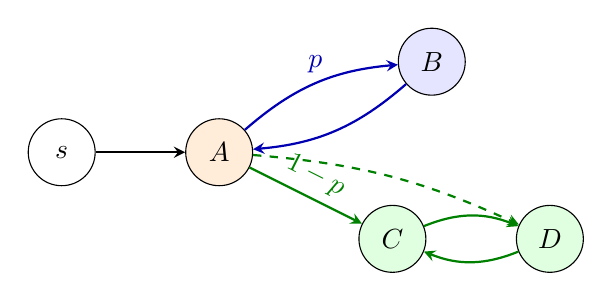
\begin{tikzpicture}[x=1cm,y=1cm,v/.style={draw,circle,minimum size=.85cm},link/.style={-stealth,thick}]
\node[v] (s) at (0,0) {$s$};
\node[v,fill=orange!15] (A) at (2,0) {$A$};
\node[v,fill=blue!10] (B) at (4.7,1.15) {$B$};
\node[v,fill=green!12] (C) at (4.2,-1.1) {$C$};
\node[v,fill=green!12] (D) at (6.2,-1.1) {$D$};
\draw[link] (s)--(A);
\draw[link,blue!70!black] (A) to[bend left=18] node[above] {$p$} (B);
\draw[link,blue!70!black] (B) to[bend left=18] (A);
\draw[link,green!50!black] (A)--node[above,sloped] {$1-p$} (C);
\draw[link,green!50!black,dashed] (A) to[bend left=10] (D);
\draw[link,green!50!black] (C) to[bend left=22] (D);
\draw[link,green!50!black] (D) to[bend left=22] (C);
\end{tikzpicture}%
}
\end{LTR}
\caption{رفتار حدی مثال نقض. جرم $1-p$ میان دو مقصد $C,D$ تقسیم می‌شود؛ تفکیک این دو مقصد در بازنمایی برچسبی اهمیتی ندارد.}
\label{cmp:fig:ch3-geometry-nonconvex-walk}
\end{figure}

در این حالت، توزیع برچسب‌های مشاهده‌شده در چهار گام به‌ترتیب $(1,0,0)$، $(0,p,1-p)$، $(p,0,1-p)$ و $(0,p^2,1-p^2)$ است (مؤلفهٔ برچسب مبدأ همواره صفر است). بنابراین برای مؤلفه‌های برچسب $A$ و $B$ داریم
\begin{equation}\label{cmp:eq:ch3-geometry-nonconvex-curve}
Y_A(p)=\alpha_1+\alpha_3p,\qquad Y_B(p)=\alpha_2p+\alpha_4p^2.
\end{equation}
در این مثال $Y_A,Y_B$ فقط نام محلی مؤلفه‌های $\mathscr Y_s$ هستند. با حذف $p$، تصویر نگاشت روی یک کمان سهموی قرار می‌گیرد. برای دو سیاست $p_1=1/4$ و $p_2=3/4$، مؤلفهٔ نخست میانگین دو بازنمایی فقط با $p=1/2$ بازتولید می‌شود؛ اما مؤلفهٔ دوم میانگین به اندازهٔ $\alpha_4/16>0$ از $Y_B(1/2)$ بزرگ‌تر است. پس این میانگین دست‌یافتنی نیست.

اگر سیاست به گام وابسته باشد و احتمال انتخاب $a$ در بازدید دوم از $(A,a)$ را $r$ بگیریم، آنگاه $Y_A=\alpha_1+\alpha_3p$ و $Y_B=\alpha_2p+\alpha_4pr$. با تعریف $z=pr$، مجموعهٔ مجاز دقیقاً $0\le z\le p\le1$ خواهد بود و نگاشت نسبت به $(p,z)$ خطی است. در نتیجه در این مثال اثر رهاسازی زمانی کاملاً آشکار است: قید منحنی $z=p^2$ به ناحیهٔ مثلثی جریان تبدیل می‌شود.

\begin{figure}[!htbp]
\centering
\begin{LTR}
\resizebox{0.60\linewidth}{!}{%
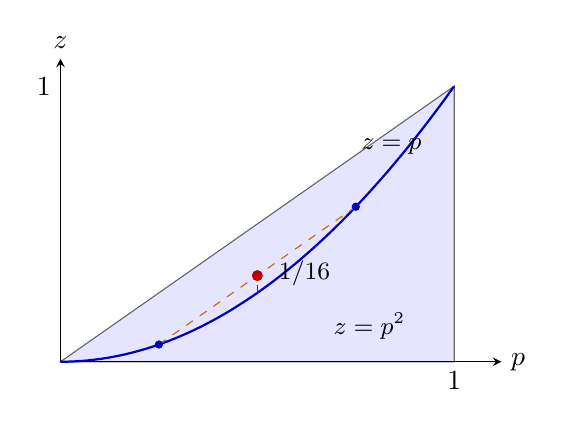
\begin{tikzpicture}[x=5cm,y=3.5cm]
\fill[blue!10] (0,0)--(1,0)--(1,1)--cycle;
\draw[black!60] (0,0)--(1,0)--(1,1)--cycle;
\draw[-stealth] (0,0)--(1.12,0) node[right] {$p$};
\draw[-stealth] (0,0)--(0,1.10) node[above] {$z$};
\draw[blue!75!black,thick,domain=0:1,samples=60] plot (\x,{\x*\x});
\draw[orange!80!black,dashed] (.25,.0625)--(.75,.5625);
\fill[blue!75!black] (.25,.0625) circle (1.5pt) (.75,.5625) circle (1.5pt);
\fill[red!75!black] (.5,.3125) circle (2pt);
\draw[red!75!black,dashed] (.5,.25)--(.5,.3125);
\node[font=\small,anchor=west] at (.53,.32) {$1/16$};
\node[font=\small,anchor=west] at (.74,.78) {$z=p$};
\node[font=\small,anchor=east] at (.9,.13) {$z=p^2$};
\node[below] at (1,0) {$1$};
\node[left] at (0,1) {$1$};
\end{tikzpicture}%
}
\end{LTR}
\caption{فضای سیاست ثابت در مثال حدی (کمان سهموی) و فضای رهاسازی زمانی (مثلث). میانگین دو نقطهٔ روی کمان الزاماً روی آن قرار نمی‌گیرد.}
\label{cmp:fig:ch3-geometry-nonconvex-curve}
\end{figure}

برای آنکه مثال نقض صرفاً به یک گراف فرضی با وزن‌های صفر متکی نباشد، آن را در گراف واقعی مدل نیز محقق می‌کنیم. مجموعه‌دادهٔ زیر را با دو ویژگی $a,b$ و چهار طبقه در نظر بگیرید؛ خط تیره نشان‌دهندهٔ ویژگی ناموجود است.
\begin{table}[!htbp]
\centering
\caption{دادهٔ مثال نقض با وزن‌های عمودی مثبت.}
\label{cmp:tab:ch3-geometry-nonconvex-data}
\begin{tabular}{c|ccc}
\hline
نمونه & $a$ & $b$ & برچسب\\\hline
$X_s$ & $0$ & -- & $1$\\
$A$ & $1$ & $R$ & $2$\\
$B$ & $R$ & -- & $3$\\
$C$ & -- & $0$ & $4$\\
$D$ & -- & $1$ & $4$\\\hline
\end{tabular}
\end{table}
در این مثال $R$ یک مقدار اسکالر محلی است، نه معیار تراکم. با متریک قدرمطلق و تابع وزن‌دهی $\kappa(r)=\exp(-r)$ و $R>2$، تمام وزن‌های عمودی مثبت، هر ویژگی در سه نمونه موجود و گراف متصل است. پس هر پنج فرض مدل برقرار است. پس از حذف $X_s$، انتقال از $A$ با ویژگی $a$ به $B$ و انتقال از $B$ به $A$ قطعی‌اند. احتمال رسیدن مستقیم از مبدأ به $B$ حداکثر $e^{1-R}$ و احتمال انتقال از $C$ یا $D$ به $A$ حداکثر $e^{2-R}$ است. شرط بر نرفتن به $A$، انتقال از $C$ به $D$ و برعکس قطعی است. در نتیجه می‌توان گشت واقعی و گشت حدی را با انتخاب‌های مشترک سیاست و انتقال، تا نخستین وقوع یکی از این رخدادهای کم‌احتمال، یکسان ساخت. احتمال تفاوت مسیر تا گام چهارم حداکثر $3e^{2-R}$ است؛ زیرا علاوه بر انتقال نخست، حداکثر دو انتقال از $C,D$ ممکن است رخ دهد. از نامنفی بودن ضرایب گام و مجموع یک آن‌ها نتیجه می‌شود که اختلاف هر مؤلفهٔ بازنمایی واقعی و حدی حداکثر
\[
\varepsilon_R=3e^{2-R}
\]
است. این کران مستقل از سیاست و در نتیجه یکنواخت است.

حتی می‌توان $R$ متناهی مشخصی ارائه کرد. برای $\beta=1/2$ و $\lambda=1$، ضرایب افق چهار برابر $(67,19,7,3)/96$ هستند. تابع سهموی در رابطه~\eqref{cmp:eq:ch3-geometry-nonconvex-curve}، به‌عنوان تابعی از مؤلفهٔ $Y_A$، روی بازهٔ مجاز دارای ثابت لیپشیتس حداکثر $L=(\alpha_2+2\alpha_4)/\alpha_3=25/7$ است. فاصلهٔ هنجار بیشینهٔ نقطهٔ میانی دو سیاست شاهد از کل کمان حدی دست‌کم
\[
\frac{\alpha_4}{16(1+L)}=\frac{7}{16384}
\]
است؛ زیرا اگر اختلاف مؤلفهٔ نخست از نقطهٔ میانی حداکثر $d$ باشد، مقدار تابع سهموی حداکثر $Ld$ از مقدار آن در مؤلفهٔ نخست نقطهٔ میانی فاصله می‌گیرد و اختلاف قائم اولیه باید حداکثر $(1+L)d$ باشد. اکنون با انتخاب $R=14$ داریم $2\varepsilon_R=6e^{-12}<7/16384$. پس میانگین دو بازنمایی واقعیِ متناظر با سیاست‌های شاهد نمی‌تواند در فضای بازنمایی‌های واقعی قرار گیرد: در غیر این صورت فاصلهٔ آن از هدف میانی حدی و فاصلهٔ بازنمایی شاهد فرضی از کمان، در مجموع حداکثر $2\varepsilon_R$ می‌شد که تناقض است. دو سیاست شاهد احتمال‌های اکیداً مثبت دارند (در سایر سطرهای دارای دو انتخاب، مثلاً احتمال‌های برابر را در نظر می‌گیریم)؛ بنابراین نامحدب بودن هم برای قرارداد بسته و هم برای قرارداد اصلی اثبات می‌شود.

از آنجا که $X_s$ تنها عضو طبقهٔ نخست است، مرکز این طبقه همان بازنمایی $\mathscr Y_s$ است. تصویر خطی یک مجموعهٔ محدب بر سطر اول باید محدب باشد؛ بنابراین نامحدب بودن مجموعهٔ بازنمایی این نمونه، نامحدب بودن فضای هم‌زمان مراکز را نیز نتیجه می‌دهد. این مثال حتی برای سیاست‌های مستقل از یکدیگر در مبدأهای مختلف برقرار است و همچنین با انتخاب سیاست‌های مشترک شاهد، برای خانوادهٔ گره‌محور مشترک برقرار می‌ماند. ازاین‌رو ثبات زمانی به‌تنهایی برای از بین رفتن تضمین عمومی محدب بودن کافی است؛ نه آنکه همهٔ نمونه‌های مسئله الزاماً فضای نامحدب داشته باشند.

\paragraph{کران‌های بلمن به‌عنوان کران‌های مختصه‌ای فضای جریان.}
فضای مراکز تحت خانوادهٔ اصلی گره‌محور مشترک را با $\mathfrak C$ (با حذف وابستگی‌های ثابت از نماد) و فضای مراکز تحت سیاست رهاسازی‌شده را با $\mathfrak C_{\mathrm{flow}}$ نشان می‌دهیم. این فضای دوم، طبق قضیهٔ~\ref{cmp:thm:ch3-geometry-flow-polytope}، چندوجهی محدب است و $\mathfrak C\subseteq\mathfrak C_{\mathrm{flow}}$ برقرار است.

کران‌های دوطرفهٔ بلمن را می‌توان از همین خانوادهٔ رهاسازی‌شده به دست آورد. برای مبدأ $s$ و مؤلفهٔ برچسب $u$، پاداش مشاهدهٔ گام $t$ را $\alpha_t^{(H)}\mathbf1_{\{y_i=u\}}$ قرار می‌دهیم. با شرط پایانی $G^{\pm}_{s,u,H+1}=0$، بازگشت بلمن عبارت است از
\begin{equation}\label{cmp:eq:ch3-bellman-value-recursion}
\begin{aligned}
G^-_{s,u,t}(i,a)&=\alpha_t^{(H)}\mathbf1_{\{y_i=u\}}+\min_{b\in A_{X_i}}\sum_{j\ne i,s}q_b^{(s)}(j\mid i)G^-_{s,u,t+1}(j,b),\\
G^+_{s,u,t}(i,a)&=\alpha_t^{(H)}\mathbf1_{\{y_i=u\}}+\max_{b\in A_{X_i}}\sum_{j\ne i,s}q_b^{(s)}(j\mid i)G^+_{s,u,t+1}(j,b).
\end{aligned}
\end{equation}
در گام پایانی جملهٔ ادامه صفر است. از آنجا که برای هر حالت، امید ادامه نسبت به توزیع احتمال اعمال خطی است، کمینه و بیشینه با انتخاب یک ویژگی مجاز نیز قابل حصول است. با استقرای معکوس، بازگشت فوق کمینه و بیشینهٔ واقعی پاداش مورد انتظار در خانوادهٔ رهاسازی‌شده را محاسبه می‌کند. با تعریف اختصاری $B_b(s,j):=q_b(j\mid s)$ برای هستهٔ نخستین انتقال، و اعمال همین انتخاب برای نخستین حرکت، داریم
\begin{equation}\label{cmp:eq:ch3-bellman-origin-bounds}
\begin{aligned}
\ell_{s,u}&=\min_{b\in A_{X_s}}\sum_{j\ne s}q_b(j\mid s)G^-_{s,u,1}(j,b),\\
U_{s,u}&=\max_{b\in A_{X_s}}\sum_{j\ne s}q_b(j\mid s)G^+_{s,u,1}(j,b).
\end{aligned}
\end{equation}
بنابراین $\ell_{s,u}$ و $U_{s,u}$ به‌ترتیب اکسترم‌های مختصهٔ $u$ از بازنمایی $\mathscr Y_s$ در خانوادهٔ رهاسازی‌شده‌اند. چون در این خانواده مبدأهای مختلف می‌توانند سیاست مستقل داشته باشند، کمینه و بیشینهٔ هر مؤلفهٔ مرکز به‌ترتیب برابر میانگین کمینه‌ها و بیشینه‌های متناظر اعضای طبقه هستند. در نتیجه
\begin{equation}\label{cmp:eq:ch3-center-component-upper}
\boxed{\begin{aligned}
L_{c,u}&=\frac1{|C_c|}\sum_{s\in C_c}\ell_{s,u}=\min_{\mathcal V\in\mathfrak C_{\mathrm{flow}}}\mathcal V_{c,u},\\
\overline U_{c,u}&=\frac1{|C_c|}\sum_{s\in C_c}U_{s,u}=\max_{\mathcal V\in\mathfrak C_{\mathrm{flow}}}\mathcal V_{c,u}.
\end{aligned}}
\end{equation}
به این ترتیب، کران‌های بلمن برای هر مختصهٔ فضای جریان تیز هستند. مجموعهٔ حاصل از اشتراک کوچک‌ترین جعبهٔ مختصه‌ای محاط‌کنندهٔ این فضا با فضای محیط مراکز را به‌صورت
\begin{equation}\label{cmp:eq:ch3-geometry-bellman-outer}
\mathfrak C_{\mathrm{Bellman}}=\{\mathcal V\in(\Delta_K)^K:L_{c,u}\le\mathcal V_{c,u}\le\overline U_{c,u}\ \forall c,u\}
\end{equation}
تعریف می‌کنیم. در نتیجه $\mathfrak C_{\mathrm{flow}}\subseteq\mathfrak C_{\mathrm{Bellman}}$. بااین‌حال، تیز بودن هر کران به‌طور جداگانه به معنای آن نیست که هر ترکیب از مقادیر مجاز مختصات را بتوان به‌طور هم‌زمان ایجاد کرد.

برای نمونه، در افق $H=1$ فرض کنیم طبقهٔ نخست فقط یک عضو $X_s$ دارد و دو ویژگی موجود در این نمونه توزیع‌های برچسبی مقصد
\[
v_1=(0,0.2,0.3,0.5),\qquad v_2=(0,0.5,0.2,0.3)
\]
را ایجاد می‌کنند. این توزیع‌ها در گراف واقعی مدل نیز قابل تحقق‌اند: کافی است سه نمونهٔ دیگر به‌ترتیب دارای برچسب‌های $2,3,4$ باشند، هر چهار نمونه هر دو ویژگی را داشته باشند، مقدار ویژگی در مبدأ صفر باشد و در سه مقصد برای هر ویژگی مقادیر $-\log v_{b,u}$، به ازای $u=2,3,4$، قرار گیرد. با متریک قدرمطلق و وزن نمایی، وزن‌های مقصد همان احتمال‌های داده‌شده‌اند و تمام فرض‌های گراف برقرارند. فضای دقیق مرکز نخست پاره‌خط $\operatorname{conv}\{v_1,v_2\}$ است. هدف $(0,0.3,0.3,0.4)$ تمام کران‌های مؤلفه‌ای بلمن را رعایت می‌کند، اما روی پاره‌خط نیست: مؤلفهٔ سوم برابر $0.3$ تنها در نقطهٔ $v_1$ حاصل می‌شود و مؤلفهٔ دوم در آن نقطه $0.2$ است. پس شمول فضای جریان در فضای بلمن ممکن است اکید باشد. این مثال با دو طبقه به همین صورت قابل ایجاد نیست، زیرا برای یک مرکز دودویی، تعیین بازهٔ یک مؤلفه، مؤلفهٔ دیگر را نیز تعیین می‌کند.

\paragraph{وابستگی کران‌ها به داده و کران پایین خطای بازیابی.}
مجموعهٔ واقعی مراکز $\mathfrak C_{\beta,\lambda,H}$ در رابطه~\eqref{cmp:eq:ch3-attainable-centers} به \emph{دادهٔ مرجع، وزن‌های گراف و خانوادهٔ سیاست} وابسته است. با آشکارکردن این وابستگی‌ها، همان مجموعه را چنین می‌نویسیم:
\begin{equation}\label{cmp:eq:ch3-attainable-centers-data-explicit}
\mathfrak R(D;\beta,\lambda,H,\mathcal Z)
=\{\mathcal V(z;D,\beta,\lambda,H):z\in\mathcal Z\}.
\end{equation}
تمام اعضای این مجموعه در بازه‌های ضروری رابطه~\eqref{cmp:eq:ch3-center-component-upper} قرار می‌گیرند. نه دست‌یافتنی‌بودن هدف بیزی در یک داده به همهٔ داده‌ها تعمیم دارد و نه برابرشدن مراکز بیزی و گشت، برابری پسین‌های نمونه‌ای یا بهبود دقت متوازن را تضمین می‌کند.

برای هدف $p=\mathcal V_c^\star$، اگر مختصهٔ $u$ بیرون بازهٔ $[L_{c,u},\overline U_{c,u}]$ باشد، برای هر مرکز مجاز $q$ از نامساوی داده‌پردازی و کران پینسکر با لگاریتم طبیعی نتیجه می‌شود
$\operatorname{JSD}(p,q)\ge \frac12\operatorname{dist}(p_u,[L_{c,u},\overline U_{c,u}])^2$.
صورت دقیق‌تر برنولی در پیوست اثبات شده است و \emph{کران‌های یک سطر را نمی‌توان بدون برهان روی مختصات جمع کرد.}
این قضیه در حساب دقیق برقرار است؛ تفسیر خروجی محاسبات شناور به‌عنوان گواه قطعی، مستلزم محصورسازی مستقل خطای هسته، ضرایب، بازگشت‌ها و هدف است. صرف شکست حلگر یا مشاهده شکاف در \lr{float64} چنین گواهی نیست.

\paragraph{بلمن در جهت‌های عمومی و تابع تکیه‌گاه.}
محدودیت آزمون مؤلفه‌ای از انتخاب پاداش‌های یک‌مختصه‌ای ناشی می‌شود، نه از خود بازگشت بلمن. برای بردار دلخواه $w\in\mathbb R^K$، پاداش گام $t$ را برابر $\alpha_t^{(H)}w_{y_i}$ قرار می‌دهیم. با شرط $G^+_{s,w,H+1}=0$، بازگشت بیشینه عبارت است از
\begin{equation}\label{cmp:eq:ch3-geometry-directional-bellman}
G^+_{s,w,t}(i,a)=\alpha_t^{(H)}w_{y_i}+\max_{b\in A_{X_i}}\sum_{j\ne i,s}q_b^{(s)}(j\mid i)G^+_{s,w,t+1}(j,b).
\end{equation}
به همان استدلال استقرای معکوس، اکسترم جهت $w$ در فضای بازنمایی نمونه برابر است با
\begin{equation}\label{cmp:eq:ch3-geometry-directional-origin}
\max_{b\in A_{X_s}}\sum_{j\ne s}q_b(j\mid s)G^+_{s,w,1}(j,b).
\end{equation}
با میانگین‌گیری این مقادیر روی اعضای طبقه، تابع تکیه‌گاه فضای مراکز رهاسازی‌شدهٔ همان طبقه حاصل می‌شود:
\begin{equation}\label{cmp:eq:ch3-geometry-support-function}
h_c(w)=\frac1{|C_c|}\sum_{s\in C_c}\max_{b\in A_{X_s}}\sum_{j\ne s}q_b(j\mid s)G^+_{s,w,1}(j,b)
=\max_{v\in\mathfrak C_{\mathrm{flow},c}}\langle w,v\rangle,
\end{equation}
که $\mathfrak C_{\mathrm{flow},c}$ تصویر $\mathfrak C_{\mathrm{flow}}$ روی سطر $c$ است. چون سیاست‌های مبدأهای متفاوت در خانوادهٔ رهاسازی‌شده مستقل‌اند، $\mathfrak C_{\mathrm{flow}}=\prod_c\mathfrak C_{\mathrm{flow},c}$ نیز برقرار است. طبق قضیهٔ جداسازی مجموعه‌های محدب بسته، داریم
\begin{equation}\label{cmp:eq:ch3-geometry-support-characterization}
\boxed{\mathcal V^\star\in\mathfrak C_{\mathrm{flow}}\iff\forall c,\ \forall w\in\mathbb R^K:\ \langle w,\mathcal V_c^\star\rangle\le h_c(w).}
\end{equation}
اگر هدف به یکی از مجموعه‌های محدب سطری تعلق نداشته باشد، قضیهٔ جداسازی وجود جهتی را تضمین می‌کند که نامساوی فوق را نقض می‌کند. در جهت دیگر، هر عضو مجموعه مطابق تعریف تابع تکیه‌گاه تمام نامساوی‌ها را رعایت می‌کند. کران‌های قبلی بلمن با محدود کردن $w$ به جهت‌های $\pm e_u$ حاصل می‌شوند. افزودن جهت‌های بیشتر، مجموعهٔ بیرونی را تنگ‌تر می‌کند و بررسی تمام جهت‌ها دقیقاً همان فضای جریان را توصیف می‌کند. بدین ترتیب برنامه‌ریزی خطی جریان و بلمن در جهت‌های عمومی دو نمایش مکمل از یک هندسهٔ محدب‌اند: اولی برای بررسی هم‌زمان یک هدف و استخراج سیاست رهاسازی‌شده مناسب است و دومی برای محاسبهٔ مرز در جهت‌های مشخص.

\begin{figure}[!htbp]
\centering
\begin{LTR}
\resizebox{0.67\linewidth}{!}{%
\begin{tikzpicture}[x=1cm,y=1cm]
\draw[black!65] (0,5)--(-2.9,0)--(2.9,0)--cycle;
% A schematic flow polytope and its coordinate box intersected with the simplex.
\filldraw[fill=black!5,draw=black!55,dashed] (-1.9,.55)--(-1.9,1.05)--(-.65,3.2)--(.45,3.2)--(1.75,.95)--(1.75,.55)--cycle;
\filldraw[fill=blue!14,draw=blue!70!black,thick] (-1.9,.55)--(-.65,3.2)--(.45,2.45)--(1.75,.95)--(.55,.55)--cycle;
\filldraw[fill=green!25,draw=green!50!black] (-.65,1.2)--(-.45,1.85)--(.1,1.35)--cycle;
\filldraw[fill=green!25,draw=green!50!black] (.42,1.0)--(.75,1.35)--(1.02,1.02)--cycle;
\fill[red!75!black] (1.4,.61) circle (2.5pt);
\node[font=\small,anchor=west,text=red!75!black] at (1.52,.45) {\rl{هدف ردشده با جریان}};
\node[font=\small,text=blue!70!black] at (-.6,2.35) {\rl{فضای جریان}};
\node[font=\small] at (.1,3.43) {\rl{کران بلمن}};
\node[font=\small,anchor=east,text=green!50!black] at (-.80,1.38) {\rl{کران داخلی}};
\node[above] at (0,5) {$e_1$};
\node[below left] at (-2.9,0) {$e_2$};
\node[below right] at (2.9,0) {$e_3$};
\end{tikzpicture}%
}
\end{LTR}
\caption{نمای شماتیک کران‌های داخلی و بیرونی. چندوجهی جریان فضای دقیق خانوادهٔ رهاسازی‌شده است و کران‌های مؤلفه‌ای بلمن ممکن است بزرگ‌تر باشند. شکل فضای واقعی سیاست در این نمودار تعیین نشده است.}
\label{cmp:fig:ch3-geometry-flow-bellman-bounds}
\end{figure}

\paragraph{جمع‌بندی کران‌های دست‌یابی.}
برای ساخت یک کران داخلی، یک یا چند سیاست میانی مجاز را ثابت نگه می‌داریم و برای هر یک از آن‌ها فضای دست‌یافتنی از طریق تغییر سیاست آغاز را طبق رابطه~\eqref{cmp:eq:ch3-geometry-center-minkowski} تعیین می‌کنیم. اجتماع این فضاها (با درون نسبی آن‌ها در قرارداد اصلی) را با $\mathfrak C_{\mathrm{in}}$ نشان می‌دهیم. برخلاف هر چندوجهی حاصل از تثبیت یک سیاست میانی، این اجتماع الزاماً محدب نیست و گرفتن پوش محدب آن بدون اثبات اضافی مجاز نیست؛ زیرا میانگین مراکز دو سیاست متفاوت ممکن است تحت یک سیاست ثابت در طول گشت دست‌یافتنی نباشد.
\begin{equation}\label{cmp:eq:ch3-geometry-attainability-sandwich}
\boxed{\mathfrak C_{\mathrm{in}}\subseteq\mathfrak C\subseteq\mathfrak C_{\mathrm{flow}}\subseteq\mathfrak C_{\mathrm{Bellman}}.}
\end{equation}
در نتیجه، اگر هدف در کران داخلی قرار گیرد، دست‌یابی به آن اثبات شده است. اگر هدف خارج از فضای جریان قرار گیرد، دست‌نیافتنی بودن آن در خانوادهٔ اصلی اثبات می‌شود؛ خارج بودن از کران بلمن نیز برای این حکم کافی است. برای اهدافی که در فضای جریان قرار دارند ولی عضویت آن‌ها در فضای واقعی معلوم نیست، به بررسی قیود سیاست یا حل مسئلهٔ معکوس نیاز داریم. اگر از یک تابع زیان نامنفی مانند مجموع وزن‌دار JSD با وزن‌های مثبت استفاده شود، کمینهٔ آن روی چندوجهی جریان، کران پایین خطای بهینهٔ خانوادهٔ اصلی است. این کمینه روی مجموعهٔ فشردهٔ جریان حاصل می‌شود و برای هدف خارج از آن اکیداً مثبت است. بدین ترتیب می‌توان میان شکست یک حلگر نامحدب و عدم امکان ساختاری دست‌یابی تمایز قائل شد.

از نظر نظری، با افق متناهی و ضرایب جبری معلوم، مسئلهٔ دست‌یابی در خانوادهٔ گره‌محور را می‌توان به امکان‌پذیری دستگاهی از معادلات و نامعادلات چندجمله‌ای تبدیل کرد: یا مستقیماً از نگاشت چندجمله‌ای احتمال‌ها، یا از دستگاه جریان به همراه قیود درجهٔ دوم رابطه~\eqref{cmp:eq:ch3-geometry-flow-policy-sharing} استفاده می‌کنیم. امکان تصمیم‌گیری نظری برای چنین دستگاه‌هایی، به معنای وجود حلگر کارآمد برای ابعاد مسئلهٔ حاضر نیست. در این پژوهش به توصیف کران‌های فوق اکتفا می‌کنیم؛ تنگ‌تر کردن فضای بیرونی، نزدیک کردن کران‌های داخلی و بیرونی، و طراحی روش‌های محاسباتی کارآمد برای گواهی دست‌یابی، موضوع پژوهش‌های آینده‌اند.

\subsection{روندهای محاسبهٔ کران‌ها و آزمون دست‌یابی}
\label{app:geometry-attainability-algorithms}
در این قسمت دو روند محاسباتی برای گراف کامل یا تنک‌شده ارائه می‌کنیم. زیرروال~\ref{cmp:alg:ch3-build-vertical}، $\operatorname{BuildVertical}$، فهرست‌های همسایگی $N_b^{(\Delta)}(i)$ و احتمال‌های پایهٔ $\widetilde q_b$ را می‌سازد؛ اگر $\Delta\ge\max_b(|D_b|-1)$ باشد (با رعایت $\Delta>3$)، گراف کامل حفظ می‌شود. خروجی این زیرروال، همراه با $D,Y$ و بردار آمادهٔ $\boldsymbol\alpha^{(H)}$ از زیرروال~\ref{cmp:alg:ch3-capped-walk-weights}، ورودی هر دو روند است. نه $\Delta$ و نه هسته‌های وابسته به مبدأ، ورودی مستقل این دو روند نیستند.

برای هر مبدأ $s$، زیرروال~\ref{cmp:alg:ch3-vertical-row}، $\operatorname{VerticalRow}$، مجموعهٔ مقصدهای مجاز $\mathcal J_{i,b}^{(s)}$ و احتمال‌های $\bar q_b^{(s)}$ را از همان هستهٔ پایه استخراج می‌کند. مطابق رابطه~\eqref{cmp:eq:ch3-sparse-vertical-transition}، حذف مبدأ و نرمال‌سازی مجدد فقط در صورت وجود مبدأ در فهرست همسایگی لازم است. حافظهٔ موقت $\mathcal C_s$ در آغاز پردازش هر مبدأ تهی است. نخستین انتقال مستقیماً از $\widetilde q_b(j\mid s)$ استفاده می‌کند. تمام استدلال‌های جریان و بلمن برای هر گراف منتخب ثابت نیز برقرارند؛ حداقل درجهٔ دو ناتهی بودن مقصدها پس از حذف مبدأ را تضمین می‌کند. کران‌های حاصل برای همان گراف منتخب معتبرند و تغییر $\Delta$ لزوماً مجموعه‌های دست‌یافتنی تودرتو ایجاد نمی‌کند.

\paragraph{محاسبهٔ کران‌های بلمن.}
در کنترل‌گر رهاسازی‌شده، مقدار بهینهٔ ادامه به ویژگی ورودی $a$ وابسته نیست؛ زیرا اعمال مجاز، پاداش و هستهٔ عمودی برای تمام ویژگی‌های ورودی یک نمونه یکسان‌اند. ازاین‌رو در الگوریتم~\ref{cmp:alg:ch3-geometry-bellman-bounds} مقدارهای $G_i^-$ و $G_i^+$ را به‌صورت بردارهای $K$ مؤلفه‌ای نگه می‌داریم. کمینه و بیشینه در این الگوریتم مؤلفه‌به‌مؤلفه‌اند و ممکن است برای برچسب‌های متفاوت از ویژگی‌های متفاوتی حاصل شوند. مقدارهای موقت $T_{i,b}^\pm$ و $G_i^{\mathrm{new},\pm}$ از مقادیر گام بعد محاسبه می‌شوند؛ جایگزینی آرایهٔ قبلی تنها پس از تکمیل همهٔ نمونه‌ها انجام می‌شود.

\begin{algorithm}[!htbp]
\caption{روند $\operatorname{BellmanBounds}$: کران‌های دوطرفهٔ بازنمایی‌ها و مراکز}
\label{cmp:alg:ch3-geometry-bellman-bounds}
\begin{algorithmic}[1]
\REQUIRE $D,Y$؛ $N_b^{(\Delta)},\widetilde q_b$؛ $\boldsymbol\alpha^{(H)}$
\ENSURE $\ell_{s,u},U_{s,u}$ و $L_{c,u},\overline U_{c,u}$ برای همهٔ اندیس‌ها
\FOR{$s=1,\ldots,n$}
    \STATE $\mathcal C_s\gets\varnothing$
    \FORALL{$i\ne s$}
        \STATE $G_i^-\gets\alpha_H^{(H)}Y_{i,:}$؛ $G_i^+\gets G_i^-$
    \ENDFOR
    \FOR{$t=H-1,\ldots,1$}
        \FORALL{$i\ne s$ و $b\in A_{X_i}$}
            \STATE $(\mathcal J_{i,b}^{(s)},\bar q_b^{(s)})\gets\operatorname{VerticalRow}(i,b,s;N,\widetilde q,\mathcal C_s)$
            \STATE $T_{i,b}^{\pm}\gets\sum_{X_j\in\mathcal J_{i,b}^{(s)}}\bar q_b^{(s)}(j\mid i)G_j^{\pm}$
        \ENDFOR
        \FORALL{$i\ne s$}
            \STATE $G_i^{\mathrm{new},-}\gets\alpha_t^{(H)}Y_{i,:}+\min_{b\in A_{X_i}}T_{i,b}^-$
            \STATE $G_i^{\mathrm{new},+}\gets\alpha_t^{(H)}Y_{i,:}+\max_{b\in A_{X_i}}T_{i,b}^+$
        \ENDFOR
        \STATE $G^{\pm}\gets G^{\mathrm{new},\pm}$
    \ENDFOR
    \FORALL{$b\in A_{X_s}$}
        \STATE $T_{s,b}^{\pm}\gets\sum_{X_j\in N_b^{(\Delta)}(s)}\widetilde q_b(j\mid s)G_j^{\pm}$
    \ENDFOR
    \STATE $\ell_{s,:}\gets\min_{b\in A_{X_s}}T_{s,b}^-$؛ $U_{s,:}\gets\max_{b\in A_{X_s}}T_{s,b}^+$
\ENDFOR
\FOR{$c=1,\ldots,K$}
    \STATE $L_{c,:}\gets\frac1{|C_c|}\sum_{s\in C_c}\ell_{s,:}$
    \STATE $\overline U_{c,:}\gets\frac1{|C_c|}\sum_{s\in C_c}U_{s,:}$
\ENDFOR
\STATE \textbf{بازگردان} $(\ell,U,L,\overline U)$
\end{algorithmic}
\end{algorithm}

در افق $H=1$ حلقهٔ پس‌رونده اجرا نمی‌شود و کران‌ها فقط از نخستین انتقال به دست می‌آیند. برای بلمن چندجهتی نیز کافی است در همین روند، به جای بردار پاداش $Y_{i,:}$ مقدار اسکالر $w_{y_i}$ قرار گیرد. در این صورت کران بالای طبقه همان $h_c(w)$ در رابطه~\eqref{cmp:eq:ch3-geometry-support-function} و کران پایین برابر $-h_c(-w)$ خواهد بود. در گراف تنک، هزینهٔ هر گام پس‌رونده برای مبدأ $s$ از مرتبهٔ $O(K\Delta m_s)$ و هزینهٔ کل روند، بدون هزینهٔ ساخت اولیهٔ گراف، از مرتبهٔ $O(nHK\Delta m)$ است. دو لایهٔ زمانی کافی‌اند؛ آرایه‌های موقت از مرتبهٔ $O(K(n+m))$ و حافظهٔ سطرهای اصلاح‌شده حداکثر $O(\Delta m)$ است. محاسبات مبدأهای متفاوت مستقل و قابل موازی‌سازی‌اند.

\paragraph{آزمون خطی دست‌یابی به مراکز هدف.}
الگوریتم~\ref{cmp:alg:ch3-geometry-flow-attainability} از جریان تجمیع‌شدهٔ رابطه~\eqref{cmp:eq:ch3-geometry-aggregated-flow} استفاده می‌کند. همهٔ متغیرهای $p,x,g$ نامنفی‌اند؛ $p$ فقط برای ویژگی‌های موجود مبدأ، $x$ فقط برای نمونه‌های غیرمبدأ و $g$ فقط برای ویژگی‌های موجود نمونه‌های غیرمبدأ تعریف می‌شوند. در شبه‌کد، افزودن قیود به معنی ساخت دستگاه خطی است، نه انتساب مقدار عددی به متغیر مجهول. برای مراکز هدف، قید برابری برای تمام طبقه‌ها و برچسب‌ها به دستگاه افزوده می‌شود. از حلگر برنامه‌ریزی خطی با تابع هدف صفر برای آزمون امکان‌پذیری استفاده می‌کنیم.

\begin{algorithm}[!htbp]
\caption{روند $\operatorname{FlowAttainability}$: آزمون خطی دست‌یابی و بازسازی سیاست رهاسازی‌شده}
\label{cmp:alg:ch3-geometry-flow-attainability}
\begin{algorithmic}[1]
\REQUIRE $D,Y$؛ $N_b^{(\Delta)},\widetilde q_b$؛ $\boldsymbol\alpha^{(H)}$؛ مراکز هدف $\mathcal V^\star$
\ENSURE وضعیت امکان‌پذیری و در صورت وجود، سیاست رهاسازی‌شده
\STATE $\mathcal C\gets\varnothing$؛ مجموعهٔ قیود خطی
\FOR{$s=1,\ldots,n$}
    \STATE $\mathcal C_s\gets\varnothing$
    \FORALL{$i\ne s$ و $b\in A_{X_i}$}
        \STATE $(\mathcal J_{i,b}^{(s)},\bar q_b^{(s)})\gets\operatorname{VerticalRow}(i,b,s;N,\widetilde q,\mathcal C_s)$
    \ENDFOR
    \STATE تعریف متغیرهای نامنفی $p_{s,b},x_{s,t}(i),g_{s,t}(i,b)$
    \STATE افزودن $\sum_{b\in A_{X_s}}p_{s,b}=1$ به $\mathcal C$
    \FORALL{$j\ne s$}
        \STATE افزودن $x_{s,1}(j)=\sum_{\substack{b\in A_{X_s}\\X_j\in N_b^{(\Delta)}(s)}}p_{s,b}\widetilde q_b(j\mid s)$
    \ENDFOR
    \FOR{$t=1,\ldots,H-1$}
        \FORALL{$i\ne s$}
            \STATE افزودن $\sum_{b\in A_{X_i}}g_{s,t}(i,b)=x_{s,t}(i)$
        \ENDFOR
        \FORALL{$j\ne s$}
            \STATE افزودن $x_{s,t+1}(j)=\sum_{\substack{i\ne s,\ b\in A_{X_i}\\X_j\in\mathcal J_{i,b}^{(s)}}}g_{s,t}(i,b)\bar q_b^{(s)}(j\mid i)$
        \ENDFOR
    \ENDFOR
    \STATE $\mathscr Y_s\gets\sum_{t=1}^H\alpha_t^{(H)}\sum_{i\ne s}x_{s,t}(i)Y_{i,:}$ \COMMENT{عبارت خطی}
\ENDFOR
\FOR{$c=1,\ldots,K$}
    \STATE افزودن $\sum_{s\in C_c}\mathscr Y_s=|C_c|\mathcal V_c^\star$ به $\mathcal C$
\ENDFOR
\STATE $(\mathrm{status},p,x,g)\gets\operatorname{SolveLP}(\min 0;\mathcal C)$
\IF{$\mathrm{status}\ne\mathrm{FEASIBLE}$}
    \STATE \textbf{بازگردان} $\mathrm{status}$ \COMMENT{ناسازگار یا نامعین}
\ENDIF
\STATE $\pi(b\mid s,\bot)\gets p_{s,b}$ برای تمام $s,b\in A_{X_s}$
\FORALL{$s,\ 1\le t<H,\ i\ne s,\ b\in A_{X_i}$}
    \STATE $\pi_{s,t}(b\mid i,a)\gets\begin{cases}g_{s,t}(i,b)/x_{s,t}(i)&x_{s,t}(i)>0,\\1/d_i&x_{s,t}(i)=0\end{cases}$ برای هر $a\in A_{X_i}$
\ENDFOR
\STATE \textbf{بازگردان} $(\mathrm{FEASIBLE},\pi,\{\pi_{s,t}\})$
\end{algorithmic}
\end{algorithm}

در حساب دقیق، وضعیت ناسازگار بودن دستگاه گواه دست‌نیافتنی بودن هدف در خانوادهٔ اصلی است. وضعیت سازگار فقط وجود جواب در خانوادهٔ رهاسازی‌شده را تضمین می‌کند؛ برای اثبات دستیابی در خانوادهٔ اصلی باید سیاست شاهد قیود مشترک بودن، ثبات زمانی و مثبت بودن احتمال‌های مجاز را نیز ارضا کند. شکست عددی حلگر یا پایان یافتن مهلت اجرا باید با وضعیت نامعین گزارش شود، نه ناسازگار. در عمل، کنترل مستقل باقیماندهٔ قیود و گواه دوگان با لحاظ خطای ضرایب برای نتیجه‌گیری قطعی لازم است. ضرایب انتقال دستگاه به‌صورت تنک از فهرست‌های خروجی $\mathcal J_{i,b}^{(s)}$ درج می‌شوند. بخش انتقال دستگاه برای هر مبدأ و هر گام حداکثر $O(\Delta m_s)$ ضریب ناصفر دارد؛ این کران مربوط به ساخت و ذخیرهٔ قیود است، نه زمان حل برنامهٔ خطی.

\paragraph{مقایسهٔ عددی دو روند.}
با حذف قیود مرکز هدف از دستگاه خطی، می‌توان برای هر $(c,u)$ دو برنامهٔ خطی با تابع هدف $\mathcal V_{c,u}=|C_c|^{-1}\sum_{s\in C_c}\mathscr Y_{s,u}$، یکی کمینه‌سازی و دیگری بیشینه‌سازی، حل کرد. با گراف منتخب و وزن‌های یکسان در هر دو روند، طبق رابطه~\eqref{cmp:eq:ch3-center-component-upper}، مقدارهای بهینه باید در حساب دقیق با $L_{c,u}$ و $\overline U_{c,u}$ برابر باشند. این برابری آزمونی مستقل برای صحت پیاده‌سازی هر دو روند فراهم می‌کند. برای محاسبهٔ صرف کران‌های مختصه‌ای، اجرای بازگشت بلمن کافی است؛ دستگاه جریان زمانی ضرورت پیدا می‌کند که امکان ایجاد هم‌زمان یک هندسهٔ هدف بررسی شود. با توجه به استقلال مبدأها در رهاسازی، دستگاه هدف را نیز می‌توان به زیرمسئله‌های مستقل طبقه‌ای تفکیک کرد.
